\documentclass{report}

\usepackage[dvipsnames,x11names]{xcolor}
\usepackage[utf8]{inputenc}
\usepackage[T1]{fontenc}
\usepackage[british]{babel}
\usepackage{etoolbox}
\newbool{isRelease}
\IfFileExists{.isRelease}{\booltrue{isRelease}}{\boolfalse{isRelease}}
\usepackage[margin=2.5cm]{geometry}
\usepackage{amssymb, latexsym, mathtools}
\usepackage{times}
\usepackage{float}
\usepackage{listings}
\usepackage{natbib}
\usepackage{framed}
\ifbool{isRelease}
    {\usepackage[disable]{todonotes}}
    {\usepackage{todonotes}}

\usepackage{amsmath}
\usepackage{stmaryrd}
\usepackage{colonequals}

\usepackage{tikz}
\usetikzlibrary{automata, positioning, arrows}
\tikzset{
    state/.style={
           rectangle,
           rounded corners,
           draw=black, very thick,
           minimum height=2em,
           inner sep=2pt,
           text centered,
           },
}


\usepackage{microtype}
\usepackage{graphicx}

\usepackage[colorlinks,citecolor=blue,linkcolor=blue,anchorcolor=blue,urlcolor=blue]{hyperref}
\usepackage[capitalise,noabbrev,nameinlink]{cleveref}

\usetikzlibrary{arrows}

\newcommand{\coot}[1]{\textcolor{violet}{\emph{#1}}}
\newcommand{\njd}[1]{\textcolor{purple}{\emph{#1}}}
\newcommand{\avieth}[1]{\textcolor{blue}{\emph{#1}}}
\newcommand{\dcoutts}[1]{\textcolor{orange}{\emph{#1}}}
\addtolength{\marginparwidth}{-0.1\marginparwidth}

\newcommand{\var}[1]{\mathit{#1}}
\newcommand{\type}[1]{\mathsf{#1}}
\newcommand{\powerset}[1]{\mathbb{P}(#1)}
\newcommand{\order}[1]{\mathcal{O}\left(#1\right)}
\newcommand{\restrictdom}{\lhd}
\newcommand{\subtractdom}{\mathbin{\slashed{\restrictdom}}}
\newcommand{\restrictrange}{\rhd}

\ifbool{isRelease}
       {
         \newcommand{\hsref}[1]{}
         \newcommand{\wip}[1]{}
         \newcommand{\hide}[1]{}
       }
       {
         \newcommand{\hsref}[1]
                    {\href{https://github.com/input-output-hk/ouroboros-network/blob/master/#1}
                      {\emph{Haskell source: #1}}}
         \newcommand{\wip}[1]{\color{magenta}{#1}\color{black}}
         \newcommand{\hide}[1]{}
       }
\newcommand{\trans}[1]{\texttt{#1}}
\newcommand{\state}[1]{\texttt{#1}}
\newcommand{\msg}[1]{\texttt{#1}}
\newcommand{\Idle}{\state{Idle}}
\newcommand{\Busy}{\state{Busy}}
\newcommand{\Done}{\state{Done}}
\newcommand{\MsgDone}{\msg{MsgDone}}

% TODO: the document is using `\langle` and `\rangle` to denote lists, maybe
% it's better to use Haskell notation, will it be more in sync with other docs
% produced by the formal method team?
\renewcommand{\langle}{[}
\renewcommand{\rangle}{]}

\DeclareMathOperator{\dom}{dom}
\DeclareMathOperator{\range}{range}
\DeclareMathOperator*{\argmin}{arg\,min} % thin space, limits underneath in displays
\DeclareMathOperator*{\minimum}{min}
\DeclareMathOperator*{\maximum}{max}

% ---- Connection Manager things
\lstset{
  xleftmargin=2pt,
  stepnumber=1,
  belowcaptionskip=\bigskipamount,
  captionpos=b,
  escapeinside={*'}{'*},
  language=haskell,
  tabsize=2,
  emphstyle={\bf},
  commentstyle=\it,
  stringstyle=\mdseries\rmfamily,
  showspaces=false,
  keywordstyle=\bfseries\rmfamily,
  columns=flexible,
  basicstyle=\small\sffamily,
  showstringspaces=false,
  morecomment=[l]\%,
}

\definecolor{shadecolor}{rgb}{.6,0.6,0.8}
\usetikzlibrary{arrows,calc,matrix,shapes}
\tikzset{every scope/.style={>=triangle 60,thick}}
\exhyphenpenalty 10000

% -------

\raggedbottom

\begin{document}

\title{The Shelley Networking Protocol \\
  {\small (Version 1.0.0 , Revision \input{revisioncount})} \\
  {\large \sc An IOHK technical report}}
\author{Duncan Coutts \\ {\small \texttt{duncan@well-typed.com}} \\
                         {\small \texttt{duncan.coutts@iohk.io}}
   \and Alex Vieth \\ {\small \texttt{alex@well-typed.com}}
   \and Neil Davies \\ {\small \texttt{neil.davies@pnsol.com}} \\
                       {\small \texttt{neil.davies@iohk.io}}
   \and Marcin Szamotulski \\ {\small \texttt{marcin.szamotulski@iohk.io}}
   \and Karl Knutsson \\ {\small \texttt{karl.knutsson@iohk.io}}
   \and Marc Fontaine \\ {\small \texttt{marc.fontaine@iohk.io}}
   }
\date{\today}

\maketitle

\begin{abstract}
  This document describes .....
\end{abstract}

\tableofcontents

\section*{Version history}

\begin{description}
\item[Version 1.0.0 Nov 2019, State machines and wire format for Ouroboros-Network-1.0.0.]
\end{description}
% \chapter{Introduction}

The Cardano Consensus and Storage layer, or \emph{the consensus layer} for
short, is a critical piece of infrastructure in the Cardano Node. It
orchestrates between the \emph{network layer} below it and the
\emph{ledger layer} above it.

The network layer is a highly concurrent piece of software that deals with
low-level concerns; its main responsibility is to transmit data efficiently
across the network. Although it primarily transmits blocks and block headers, it
does not interpret them and does not need to know much about them. In the few
cases where it \emph{does} need to make some block-specific decisions, it
calls back into the consensus layer to do so.

The ledger layer by contrast exclusively deals with high-level concerns. It is
entirely stateless: its main responsibility is to define a single pure
function describing how the ledger state is transformed by blocks (verifying
that blocks are valid in the process). It is only concerned with linear history;
it is not aware of the presence of multiple competing chains or the roll backs
required when switching from one chain to another. We do require that the ledger
layer provides limited \emph{lookahead}, computing (views on near)
\emph{future} ledger states (required to be able to validate block headers
without access to the corresponding block bodies)

The consensus layer mediates between these two layers. It includes a
bespoke storage layer that provides efficient access to the current ledger state
as well as recent \emph{past} ledger states (required in order to be able
to validate and switch to competing chains). The storage layer also
provides direct access to the blocks on the blockchain itself, so that they can
be efficiently streamed to clients (via the network layer). When there are
competing chains, the consensus layer decides which chain is preferable and
should be adopted, and it decides when to \emph{contribute} to the chain
(produce new blocks). All ``executive decisions'' about the chain are made in
and by the consensus layer.

Lastly, as well we see, the consensus layer is highly abstract and places a
strong emphasis on compositionality, making it usable with many different
consensus algorithms and ledgers. Importantly, compositionality enables the
\emph{hard fork combinator} to combine multiple ledgers and regard them as a
single blockchain.

The goal of this document is to outline the design goals for the consensus
layer, how we achieved them, and where there is still scope for improvement. We
will both describe \emph{what} the consensus layer is, and \emph{why} it is the
way it is. Throughout we will also discuss what \emph{didn't} work, approaches
we considered but rejected, or indeed adopted but later abandoned; discussing
these dead ends is sometimes at least as informative as discussing the solution
that did work.

We will consider some of the trade-offs we have had to make, how they
affected the development, and discuss which of these trade-offs should perhaps
be reconsidered. We will also take a look at how the design can scale to
facilitate future requirements, and which requirements will be more problematic
and require more large-scale refactoring.

The target audience for this document is primarily developers working on the
consensus layer. It may also be of more broader interest to people generally
interested in the Cardano blockchain, although we will assume that the
reader has a technical background.

\chapter{System Architecture}

\section{Data Flow in a Node}
Nodes maintain connections with the peers that have been chosen
with help of the peer selection process.
Suppose node $A$ is connected to node $B$.
The Ouroboros protocol schedules a node $N$ to generate a new block in a given time slot.
Depending on the location of nodes $A$, $B$ and $N$ in the network topology and whether the new
block arrives first at $A$ or $B$, $A$ can be either up-stream or down-stream of $B$.
Therefore, node $A$ runs an instance of the client side of the chain-sync mini protocol
that talks with a server instance of chain-sync at node $B$ and also a server instance of chain sync
that talks with a client instance at $B$.
The situation is similar for the other mini protocols (block fetch, transaction submission, etc).
The set of mini protocols that runs over a connection is determined by the version of the network
protocol, i.e.  Node-to-Node, Node-to-Wallet and Node-to-Chain-Consumer
connections use different sets of mini protocols (e.g. different protocol
versions).  The version is negotiated when a new connection is established
using protocol which is described in Chapter~\ref{connection-management}.
\hide{Add description of this protocol in Chapter~\ref{connection-management}
and link it.}

\begin{figure}[ht]
  \pgfdeclareimage[height=15cm]{node-diagram-chains-state}{figure/node-diagram-concurrency.pdf}
  \begin{center}
    \pgfuseimage{node-diagram-chains-state}
  \end{center}
  \caption{Data flow inside a Node}
  \label{node-diagram-concurrency}
\end{figure}

Figure~\ref{node-diagram-concurrency} illustrates parts of the data flow in a node.
Circles represents a thread that runs one of the mini protocols (the mini protocols are explained in
Chapter~\ref{state-machine-section}).
There are two kinds of data flows:
mini protocols communicate with mini protocols of other nodes by sending and receiving messages;
and, within a node, they communicate by reading from- and writing to- a shared
mutable variable, which are represented by boxes in
Figure~\ref{node-diagram-concurrency}.
\href{https://en.wikipedia.org/wiki/Software_transactional_memory}{Software transactional memory}
(STM) is a mechanism for safe and lock-free concurrent
access to mutable state and the reference implementation makes intensive use of
this abstraction (see \cite{stm:harris2006}).

\section{Congestion Control}
A central design goal of the system is robust operation at high workloads.
For example, it is a normal working condition of the networking design
that transactions arrive at a higher rate than the number
that can be included in blockchain.
An increase of the rate at which transactions are submitted must not cause a decrease
of the block chain quality.

Point-to-point TCP bearers do not deal well with overloading.
A TCP connection has a certain maximal bandwidth,
i.e. a certain maximum load that it can handle relatively reliably under normal conditions.
If the connection is ever overloaded,
the performance characteristics will degrade rapidly unless
the load presented to the TCP connection is appropriately managed.

At the same time, the node itself has a limit on the rate at which it can process data.
In particular, a node may have to share its processing power with other processes that run on the
same machine/operation system instance, which means that a node may get slowed down for some reason,
and the system may get in a situation
where there is more data available from the network than the node can process.
The design must operate appropriately in this situation and recover form transient conditions.
In any condition, a node must not exceed its memory limits,
that is there must be defined limits, breaches of which being treated like protocol violations.

Of cause it makes no sense if the system design is robust,
but so defensive that it fails to meet performance goals.
An example would be a protocol that never transmits a message unless it has received an
explicit ACK for the previous message. This approach might avoid overloading the network,
but would waste most of the potential bandwidth.


\section{Real-time Constraints and Coordinated Universal Time}
Ouroboros models the passage of physical time as an infinite sequence of time slots,
i.e. contiguous, equal-length intervals of time,
and assigns slot leaders (nodes that are eligible to create a new block) to those time slots.
At the beginning of a time slot, the slot leader selects the block chain and transactions that are the basis
for the new block, then it creates the new block and sends the new block to its peers.
When the new block reaches the next block leader before the beginning of next time slot,
the next block leader can extend the block chain upon this block (if the block
did not arrive on time the next leader will create a new block anyway).

There are some trade-offs when choosing the slot time that is used for the protocol but
basically the slot length should be long enough such that a new block has a good chance to reach the
next slot leader in time.
A chosen value for the slot length is 20 seconds.
It is assumed that the clock skews between the local clocks of the nodes is small with respect to the
slot length.

However, no matter how accurate the local clocks of the nodes are with respect to the time slots
the effects of a possible clock skew must still be carefully considered.
For example, when a node time-stamps incoming blocks with its local clock time, it may encounter
blocks that are created in the future
with respect to the local clock of the node.
The node must then decide whether this is because of a clock skew or whether the node considers this
as adversarial behavior of an other node.

\wip{TODO :: get feedback from the researchers on this. Tentative policy: allow 200ms to 1s
explain the problem in detail.
A node cannot forward a block from the future.
This is complicated !
}

\chapter{Mini Protocols}
\label{state-machine-section}

\section{Mini Protocols and Protocol Families}
A mini protocol is a well defined and modular building block of
the network protocol.
Structuring the protocol around mini protocols helps to manage the overall complexity of
the design and adds useful flexibility.
The design turns into a family of mini protocols that can be specialised to particular requirements
by choosing a particular set of mini protocols.

The mini protocols in this section describe both the initiator and responder of a communication.
The initiator is the dual of the responder and vice versa.
(The terms client/server and consumer/producer are also used sometimes.)
At any time a node will typically run many instances of mini protocols, including many instances of the
same mini protocol.
Each mini protocol instance of the node communicates with the dual
instance of exactly one peer.
All mini protocols that communicate with the same peer
share a single communication channel (pipe or socket)
and a multiplexer/de-multiplexer is used to multiplex the protocols over that channel.
Section~\ref{multiplexing-section} describes the multiplexing layer.

The set of mini protocols that run on a connection between two participants of the system
depends on the role of the participants, i.e. whether the node acts as a full node or just
a block chain consumer, for example a wallet.
\wip{
Section~\ref{peer-setup-section} describes how a connection between two nodes
that run a set of mini protocols is set up.
}

\section{Protocols as State Machines}
The implementation of the mini protocols uses a generic framework for state machines.
\hide{
The Haskell implementation of the state machine framework is described in
Section~\ref{Haskell-state-machine}.
}
This framework uses correct-by-construction techniques to guarantee
several properties of the protocol and the implementation.
In particular, it guarantees that there are no deadlocks.
At any time, one side has agency
(is expected to transmit the next message) and the other side is awaiting for
the message (or both sides agree that the protocol has terminated).
If either side receives a message that is not expected according to the protocol
the communication is aborted.

For each mini protocol that is based on this underlying framework the description provides the
following pieces of information:

\begin{itemize}
\item An informal description of the protocol.
\item States of the state machine.
\item The messages that are exchanged.
\item A transition graph of the global view of the state machine.
\item The client implementation of the protocol.
\item The server implementation of the protocol.
\end{itemize}

\begin{description}
\item[State Machine]
  Each mini protocol is described as a state machine.
  This document uses a simple diagram representations for state machines, and
  also includes corresponding transition tables.
  Descriptions of state machines in this section are directly derived from
  specifications of mini protocols using the state machine framework.

  The state machine framework that is used to specify the protocol can be instantiated
  with different implementations that work at different levels of abstraction
  (for example implementations used for simulation, implementations that run over virtual
  connections and implementations that actually transmit messages over the real network).


\item[States]
  States are abstract: they are not a value of some variables in a node, but
  rather describe the state of the two-party communication as whole, e.g.
  that a client is responsible for sending a particular type of message and
  the server is awaiting on it.  This, in particular, means that if the state
  machine is in a given state, both client and server are in this state.
  An additional piece of information that differentiates the roles of peers in
  a given state is agency, which describes which side is responsible for
  sending the next message.

  In the state machine framework, abstract states of a state machine are
  modelled as promoted types, so they do not correspond to any particular
  value hold by one of the peers.

  The document presents this abstract view of mini protocols and the state
  machines where the client and server are always in identical states, which
  also means that client and server simultaneously transit to new states.
  For this description network delays are not important.

  An interpretation, which is closer to the real-world implementation but
  less concise, is that there are independent client and server states
  and that transitions on either side happen independently when a message is sent or received.

\item[Messages]
  Messages exchanged by peers form edges of a state machine diagram, in other
  words they are transitions between states.
  They are elements from the set
  $$\{(label, data) \mid label \in Labels, data \in Data\}$$
  Protocols use a small set of $Labels$ typically $|Labels| \leq 10$.
  The state machine framework requires that messages can be serialised,
  transferred over the network and de-serialised by the receiver.
  The binary format for messages is described in Section~\ref{CBOR-section}.

\item[Agency]
  A node has agency if it is expected to send the next message.
  In every state (except the \Done-state) either the client or server has agency.
  In the \Done-state the protocol has terminated and neither side is expected to send any more
  messages.

\item [State machine diagrams]
      States are drawn as circles in state machine diagrams.
      States with agency at the client are drawn in green, states with agency at the server in blue and
      the \Done-state in black.
      By construction, the system is always in exactly one state,
      i.e. the client's state is always the same state as server's,
      and the colour indicates who is the agent.
      It is also important to understand that the arrows in the state transition diagram denote
      state transitions and not the direction of the message that is being transmitted.
      For the agent of the particular state the arrow means: ``send a message to the
      other peer and move to the next state''.
      For a non-agent an arrow in the diagram can be interpreted as:
      ``receive an incoming message and move to the next state''.
      This may be confusing because the arrows are labelled with the messages and
      many arrows go from a green state (client has the agency) to a blue
      state (server has the agency) or vice versa.

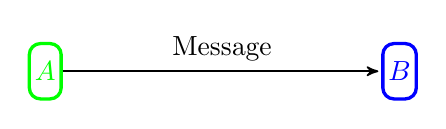
\begin{tikzpicture}[->,>=stealth',shorten >=1pt,auto,node distance=4.5cm, semithick]
  \tikzstyle{every state}=[fill=red,draw=none,text=white]
  \node[state, green]              (A)      {$A$};
  \node[state, blue ,right of=A]   (B)      {$B$};
  \draw (A)            edge[above]          node{Message}   (B);
\end{tikzpicture}

      $A$ is green, i.e in state $A$ the client has agency.
      Therefore the client sends a message to the server and
      both client and server transition to state $B$.
      As $B$ is blue the agency also changes from client to server.

\begin{tikzpicture}[->,>=stealth',shorten >=1pt,auto,node distance=4.5cm, semithick]
  \tikzstyle{every state}=[fill=red,draw=none,text=white]
  \node[state, blue]               (C)      {$C$};
  \node[state, blue ,right of=A]   (D)      {$D$};
  \draw (A)            edge[above]               node{Message}   (B);
\end{tikzpicture}

      $C$ is blue, i.e in state $C$ the server has agency.
      Therefore the server sends a message to the client and
      both client and server transition to state $D$.
      As $D$ is also blue the agency remains at the server.

\item[Client and server implementation]
  The state machine describes which messages are sent and received and in which order.
  This is the external view of the protocol that every compatible implementation MUST follow.
  In addition to the external view of the protocol, this part of the specification describes
  how the client and server actually process the transmitted messages,
  i.e. how the client and server update their internal mutable state
  upon the exchange of messages.

  Strictly speaking, the representation of the node-local mutable state
  and the updates to the node-local state are implementation details that are
  not part of the communication protocol between the nodes,  and will
  depend on an application that is built on top of the network service
  (wallet, core node, explorer, etc.).
  The corresponding sections were added to clarify the mode of operation of the
  mini protocols.

\end{description}
\section{Overview of all implemented Mini Protocols}

\newcommand{\miniEntry}[4]{
  \begin{framed}
      \noindent\textbf{#1}\hfill  Section \ref{#2}
      \newline {#3}
      \newline {\small\texttt{#4}}
  \end{framed}
}

\miniEntry
    {Ping Pong Protocol}
    {ping-pong-protocol}
    {A simple ping-pong protocol for testing.}
    {typed-protocols/src/Network/TypedProtocol/PingPong/Type.hs}

\miniEntry
    {Request Response Protocol}
    {request-response-protocol}
    {A ping pong like protocol which allows to exchanges data.}
    {typed-protocols/src/Network/TypedProtocol/ReqResp/Type.hs}

\miniEntry
    {Chain Synchronisation Protocol}
    {chain-sync-protocol}
    {The protocol by which a downstream chain consumer follows an upstream chain producer.}
    {ouroboros-network/src/Ouroboros/Network/Protocol/ChainSync/Type.hs}

\miniEntry
    {Block Fetch Protocol}
    {block-fetch-protocol}
    {The block fetching mechanism enables a node to download ranges of blocks.}
    {ouroboros-network/src/Ouroboros/Network/Protocol/BlockFetch/Type.hs}

\miniEntry
    {Local Transaction Submission Mini Protocol}
    {local-tx-submission-protocol}
    {Transmitting Transactions from a wallet to a local node.}
    {src/Ouroboros/Network/Protocol/LocalTxSubmission/Type.hs}

\miniEntry
    {Node-to-Node Transaction Submission Protocol}
    {tx-submission-protocol}
    {A Protocol for transmitting transaction between core nodes.}
    {ouroboros-network/src/Ouroboros/Network/Protocol/TxSubmission/Type.hs}

\miniEntry
    {Handshake Mini Protocol}
    {handshake-protocol}
    {This protocol is used for version negotiation.}
    {src/Ouroboros/Network/Protocol/Handshake/Type.hs}

\section{Ping-Pong Protocol}
\label{ping-pong-protocol}
\hsref{typed-protocols/src/Network/TypedProtocol/PingPong/Type.hs}
\newcommand{\Ping}{\msg{Ping}}
\newcommand{\Pong}{\msg{Pong}}

\subsection{Description}
A client can use the Ping-Pong protocol to check that the server is responsive.
The Ping-Pong protocol is very simple because the messages do not carry any data and
because the Ping-Pong client and the Ping-Pong server do not access the internal state of the node.

\subsection{State Machine}

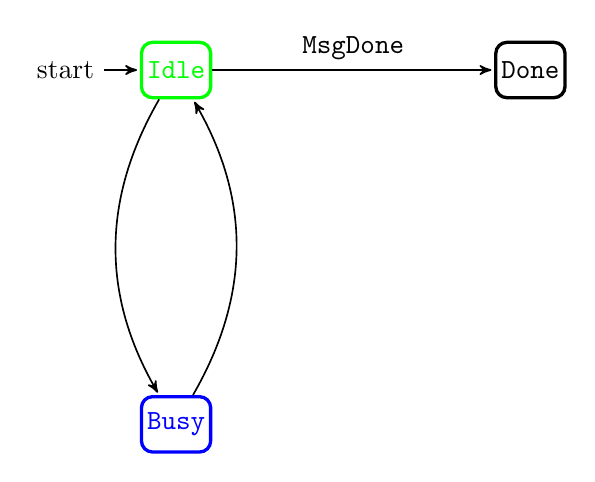
\begin{tikzpicture}[->,>=stealth',shorten >=1pt,auto,node distance=4.5cm, semithick]
  \tikzstyle{every state}=[fill=red,draw=none,text=white]
  \node[state, green, initial]                            (Idle)      {\Idle};
  \node[state, right of=Idle]                             (Done)      {\Done};
  \node[state, blue, below of=Idle]                       (Busy)      {\Busy};

  \draw (Idle)         edge[above]               node{\MsgDone}                  (Done);
  \draw (Idle)         edge[left, bend right]    node{\Ping}                     (Busy);
  \draw (Busy)         edge[right, bend right]   node{\Pong}                     (Idle);
\end{tikzpicture}

\begin{figure}[ht]
\begin{tabular}{|l|l|} \hline
\multicolumn{2}{|c|}{Agency} \\ \hline
  Client has Agency & \Idle \\  \hline
  Server has Agency & \Busy \\  \hline
\end{tabular}
\end{figure}

The protocol uses the following messages.
The messages of the Ping-Pong protocol do not carry any data.
\begin{description}
\item [\Ping]
      The client sends a Ping request to the server.
\item [\Pong]
      The server replies to a Ping with a Pong.
\item [\MsgDone]
      Terminate the protocol.
\end{description}

\begin{tabular}{|l|l|l|}
  \hline
  \multicolumn{3}{|c|}{Transition table} \\ \hline
  from state   & message            & to state    \\ \hline\hline
  \Idle        & \Ping              & \Busy   \\ \hline
  \Busy        & \Pong              & \Idle   \\ \hline
  \Idle        & \MsgDone           & \Done       \\ \hline
\end{tabular}

\section{Request Response Protocol}
\label{request-response-protocol}
\renewcommand{\Idle}{\state{Idle}}
\renewcommand{\Busy}{\state{Busy}}
\renewcommand{\Done}{\state{Done}}
\newcommand{\Request}{\msg{Request}}
\newcommand{\Response}{\msg{Response}}

\subsection{Description}
The request response protocol is polymorphic in the request and response data that is being transmitted.
This means that there are different possible applications of this protocol and the
application of the protocol determines the types of the requests and responses.

\subsection{State machine}
\hsref{ouroboros-network/src/Ouroboros/Network/Protocol/ReqResp/Type.hs}

\begin{tabular}{|l|l|}
  \hline
  \multicolumn{2}{|c|}{Agency} \\ \hline
  Client has Agency & \Idle \\  \hline
  Server has Agency & \Busy \\ \hline
\end{tabular}
{\vskip 10pt}
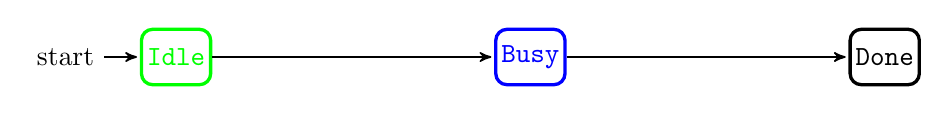
\begin{tikzpicture}[->,>=stealth',shorten >=1pt,auto,node distance=4.5cm, semithick]
  \tikzstyle{every state}=[fill=red,draw=none,text=white]
  \node[state, green, initial]                                   (Idle)      {\Idle};
  \node[state, blue, right of=Idle]                              (Busy)      {\Busy};
  \node[state, right of=Busy]                                    (Done)      {\Done};

  \draw (Idle)         edge[]      node{\Request}           (Busy);
  \draw (Busy)         edge[]      node{\Response}          (Done);
\end{tikzpicture}
{\vskip 10pt}
The protocol uses the following messages.
\begin{description}
\item [\Request{} $(request)$]
      The client sends a request to the server.
\item [\Response{} $(response)$]
      The server replies with a response.
\end{description}

\begin{tabular}{|l|l|l|l|} \hline
\multicolumn{4}{|c|}{Transition table} \\ \hline
  from         & message            & parameters             & to       \\ \hline\hline
  \Idle        & \Request           & $request$              & \Busy     \\ \hline
  \Busy        & \Response          & $response$             & \Done     \\ \hline
\end{tabular}

\section{Chain Synchronisation Protocol}
\label{chain-sync-protocol}
\hsref{ouroboros-network/src/Ouroboros/Network/Protocol/ChainSync/Type.hs}
\newcommand{\CanAwait}{\state{CanAwait}}
\newcommand{\MustReply}{\state{MustReply}}
\newcommand{\Intersect}{\state{Intersect}}
\newcommand{\RequestNext}{\msg{RequestNext}}
\newcommand{\AwaitReply}{\msg{AwaitReply}}
\newcommand{\RollForward}{\msg{RollForward}}
\newcommand{\RollBackward}{\msg{RollBackward}}
\newcommand{\FindIntersect}{\msg{FindIntersect}}
\newcommand{\IntersectFound}{\msg{IntersectFound}}
\newcommand{\IntersectNotFound}{\msg{IntersectNotFound}}

\subsection{Description}
The chain synchronisation protocol is used by a block chain consumer
to replicate the producer's block chain locally.
A node communicates with several upstream and downstream nodes
and runs an independent client instance and a independent server instance for every
other node it communicates with.
(See Figure~\ref{node-diagram-concurrency}.)

The chain synchronisation protocol is polymorphic.
The (full)-node to client protocol uses an instance of the chain synchronisation protocol
that transfers full blocks, while the node-to-node instance only transfers block headers.
In the node-to-node case, the block fetch protocol (Section \ref{block-fetch-protocol})
is used to transfer full blocks.

\subsection{State Machine}

\begin{tabular}{|l|l|}
  \hline
  \multicolumn{2}{|c|}{Agency} \\ \hline
  Client has Agency & \Idle \\  \hline
  Server has Agency & \CanAwait, \MustReply, \Intersect \\ \hline
\end{tabular}

\begin{figure}[ht]
\begin{tikzpicture}[->,>=stealth',shorten >=1pt,auto,node distance=4.5cm, semithick]
  \tikzstyle{every state}=[fill=red,draw=none,text=white]
  \node[state, green, initial]                            (Idle)      {\Idle};
  \node[state, right of=Idle]                             (Done)      {\Done};
  \node[state, blue, below left of=Idle]                  (CanAwait)  {\CanAwait};
  \node[state, blue, right of=CanAwait]                   (MustReply) {\MustReply};
  \node[state, blue, above of=Idle]                       (Intersect) {\Intersect};

  \draw (Idle)         edge[left, bend right]      node{\RequestNext}           (CanAwait);
  \draw (CanAwait)     edge[below, bend right]     node{\AwaitReply}            (MustReply);
  \draw (CanAwait)     edge[above,bend right=45]     node{\RollForward}           (Idle);
  \draw (MustReply)    edge[right,bend right=45]     node{\RollForward}           (Idle);
  \draw (CanAwait)     edge[above,bend right=80]     node{\RollBackward}          (Idle);
  \draw (MustReply)    edge[right,bend right=80]     node{\RollBackward}          (Idle);
  \draw (Idle)         edge[right, bend right]    node{\FindIntersect}         (Intersect);
  \draw (Intersect)    edge[above, bend right=45]    node[below = 4mm]{\IntersectFound}     (Idle);
  \draw (Intersect)    edge[above, bend right=80]    node[above = 4mm]{\IntersectNotFound}  (Idle);
  \draw (Idle)         edge[above]                node{\MsgDone}                  (Done);
\end{tikzpicture}
\caption{State machine of the chain sync protocol.}
\label{chain-sync-automata}
\end{figure}

The protocol uses the following messages:
\begin{description}
\item [\RequestNext]
      Request the next update from the producer.
\item [\AwaitReply]
      Acknowledge the request but require the consumer to wait for the next update.
      This means that the consumer is synced with the producer, and
      the producer is waiting for its own chain state to change.
\item [\RollForward{} {\boldmath $(header, tip)$}]
      Tell the consumer to extend their chain with the given $header$.
      The message also tells the consumer about the $tip$ of the producers chain.
\item [\RollBackward{} {\boldmath $(point_{old}, tip$}]
      Tell the consumer to roll back to a given $point_{old}$ on their chain.
      The message also tells the consumer about the current  $tip$ of the chain the producer is following.
\item [\FindIntersect{} {\boldmath $\langle point_{head} \rangle $}]
      Ask the producer to try to find an improved intersection point between
      the consumer and producer's chains.
      The consumer sends a sequence {\boldmath $\langle point \rangle $}
      and it is up to the producer
      to find the first intersection point on its chain and send it back to the consumer.
\item [\IntersectFound{} {\boldmath $(point_{intersect} ,tip)$}]
      The producer replies with the first point of the request that is on his current chain.
      The consumer can decide whether to send more points.
      The message also tells the consumer about the $tip$ of the producer.
\item [\IntersectNotFound{} {\boldmath $(tip)$}]
      The reply to the consumer that no intersection was found: none of the
      points the consumer supplied are on the producer chain.
      The message only contains the $tip$ of the producer chain.
\item [\MsgDone]
      Terminate the protocol.
\end{description}

\begin{tabular}{|l|l|l|l|}
  \hline
  \multicolumn{4}{|c|}{Transition table} \\ \hline
  from state & message             & parameters                          & to state    \\ \hline\hline
  \Idle      & \RequestNext        &                                     & \CanAwait   \\ \hline
  \Idle      & \FindIntersect      & $\langle point\rangle$              & \Intersect  \\ \hline
  \Idle      & \MsgDone            &                                     & \Done       \\ \hline
  \CanAwait  & \AwaitReply         &                                     & \MustReply  \\ \hline
  \CanAwait  & \RollForward        & $header$, $tip$                     & \Idle       \\ \hline
  \CanAwait  & \RollBackward       & $header_{old}$, $tip$                & \Idle       \\ \hline
  \MustReply & \RollForward        & $header$, $tip$                     & \Idle       \\ \hline
  \MustReply & \RollBackward       & $point_{old}$, $tip$                 & \Idle       \\ \hline
  \Intersect & \IntersectFound     & $point_{intersect}$, $tip$            & \Idle       \\ \hline
  \Intersect & \IntersectNotFound  & $tip$                               & \Idle       \\ \hline

\end{tabular}

\newcommand{\readpointer}{\emph{read-pointer}}
\subsection{Implementation of the Chain Producer}
\hide{The trade-offs between the robustness and efficiency of possible chain-sync protocols are
discussed in Section~\ref{chain-sync-discussion}.
}
This section describes a state-full implementation of a chain producer that is suitable for a setting where
the producer cannot trust the chain consumer.
An important requirement in this setting
is that a chain consumer must never be able to cause excessive resource use on the producer side.
The presented implementation meets this requirement.
It uses a constant amount of memory to store the state that the producer maintains
per chain consumer.  This protocol is only used to reproduce the producer
chain locally by consumer.  By running many instances of this protocol against
different peers, a node can reproduce chains in the network and
do chain selection which by design is not part of this protocol.
Note, that when we refer to the consumer's chain in this section, we mean
the chain that is reproduced by the consumer with the instance of
the chain-sync protocol under consideration and not the result of the chain selection algorithm.

We call the state which the producer maintains about the consumer the \readpointer{}.
The \readpointer{} basically tracks what the producer knows about the head of
the consumer's chain without storing it locally.
It points to a block on the current chain of the chain producer.
The \readpointer{}s are part of the shared state of the node (Figure~\ref{node-diagram-concurrency}) and
\readpointer{}s are concurrently updated by the thread that runs the chain-sync mini-protocol and the
chain tracking logic of the node itself.

We first describe how the mini-protocol updates a \readpointer{} and later address what happens in case
of a fork.
\subparagraph{Initializing the \readpointer{}.}
The chain producer assumes that a consumer, which has just connected,
only knows the genesis block and initialises the \readpointer{} of that consumer
with a pointer to the genesis block on its chain.

\subparagraph{Downloading a chain of blocks}
A typical situation is when the consumer follows the chain of the producer but is not yet at the head of the
chain (this also covers a consumer booting from genesis).
In this case, the protocol follows a simple, consumer-driven, request-response pattern.
The consumer sends \RequestNext{} messages to ask for the next block.
If the \readpointer{} is not yet at the head of the chain,
the producer replies with a \RollForward{} and advances the \readpointer{} to
the next block (optimistically assuming that the client will update its chain
accordingly).
The \RollForward{} message contains the next block and also the head-point of the producer.
The protocol follows this pattern until the \readpointer{} reaches the end of its chain.

\begin{figure}[ht]
\pgfdeclareimage[height=7cm]{read-pointer-consumer-driver}{figure/read-pointer-consumer-driven.pdf}
\begin{center}
\pgfuseimage{read-pointer-consumer-driver}
\end{center}
\caption{Consumer driven block download.}
\label{read-pointer-consumer-driver}
\end{figure}

\subparagraph{Producer driven updates}
If the \readpointer{} points to the end of the chain and the producer receives
a \RequestNext{}
the consumers chain is already up to date.
The producer informs the consumer with an \AwaitReply{} that no new data is available.
After receiving a \AwaitReply, the consumer just waits for a new message and the producer keeps agency.
The \AwaitReply{} switches from a consumer driven phase to a producer driven phase.

The producer waits until new data becomes available.
When a new block is available, the producer will
send a \RollForward{} message and give agency back to the consumer.
The producer can also get unblocked when its node switches to a new chain fork.

\subparagraph{Producer switches to a new fork}
The node of the chain producer can switch to a new fork at any time, independent of the
state machine.
A chain switch can cause an update of the \readpointer{},
which is part of the mutable state that is shared between the thread that runs
the chain sync protocol and the thread that implements the chain following logic of the node.
There are two cases:

1) If the \readpointer{} points to a block that is on the common prefix of the new
fork and the old fork, no update of the \readpointer{} is needed.

2) If the \readpointer{} points to a block that is no longer part of the chain that is followed by the node,
the \readpointer{} is set to the last block that is common between the new and the old chain.
The node also sets a flag that signals the chain-sync thread to send a \RollBackward{} instead
of a \RollForward.
Finally the producer thread must unblock if it is in the \MustReply{} state.

\begin{figure}[ht]
\pgfdeclareimage[height=5cm]{read-pointer-rollback}{figure/read-pointer-rollback.pdf}
\begin{center}
\pgfuseimage{read-pointer-rollback}
\end{center}
\caption{\readpointer{} update for a fork switch in case of a rollback.}
\label{read-pointer-rollback}
\end{figure}

Figure~\ref{read-pointer-rollback} illustrates a fork switch that requires an update of the \readpointer{}
for one of the chain consumers, i.e. an example for case 2.
Before the switch, the \readpointer{} of the consumer points to block $0x660f$.
The producer switches to a new chain with the head of the chain at block $0xcdf0$.
The node must update the \readpointer{} to block $0xfa40$ and the next message to the consumer
will be a \RollBackward.

Note, that a node typically communicates with several consumers. For each consumer it runs an independent
version of the chain-sync-protocol state machine in an independent thread and with its own \readpointer{}.
Each of those \readpointer{}s has to be updated independently and for each consumer
either case 1) or case 2) can apply.

\subparagraph{Consumer starts with an arbitrary fork}
Typically, the consumer already knows some fork of the block chain when it
starts to track the producer.
The protocol provides an efficient method to search for the longest common prefix (here called intersection)
between the fork of the producer and the fork that is known to the consumer.

To do so, the consumer sends a \FindIntersect{} message with a list of chain
points on the chain known to the consumer.
If the producer does not know any of the points it replies with \IntersectNotFound.
Otherwise it replies with \IntersectFound{} and the best (i.e. the newest) of the points that it knows
and also updates the \readpointer{} accordingly.
For efficiency, the consumer should use a binary search scheme to search for the longest common
prefix.

It is advised that the consumer always starts with \FindIntersect{} in a fresh connection
and it is free to use \FindIntersect{} at any time later as seems beneficial.
If the consumer does not know anything about the producer's chain,
it can start the search with the following list of points:
$\langle point(b), point(b-1), point(b-2), point(b-4), point (b-8),\ldots \rangle$
where $point(b-i)$ is the point of the $i$th predecessor of block $b$ and
$b$ is the head of the consumer fork.
Maximum depth of a fork in Ouroboros is bounded and the intersection will always be found with a small number of
iterations of this algorithm.

\subsection{Implementation of the Chain Consumer}
In principle, the chain consumer has to guard against a malicious chain producer
as much as the other way around.
However, two aspects of the protocol play in favour of the consumer here.
\begin{itemize}
  \item The protocol is basically consumer driven, i.e. the producer has no way to send unsolicited
data to the consumer (within the protocol).
  \item The consumer can verify the response data itself.
\end{itemize}
Here are some cases to consider:
\begin{description}
\item[\FindIntersect~Phase]
  The consumer and the producer play a number guessing game, so the consumer can easily detect
  inconsistent behaviour.
\item[The producer replies with a \RollForward] The consumer can verify the block itself
  with the help of the ledger layer.
  (The consumer may need to download the block first, if the protocol only sends block headers.)
\item[The producer replies with a \RollBackward] The consumer tracks several producers, so
  if the producer sends false \RollBackward{} messages the consumer's node
  will, at some point, just switch to a longer chain fork.
\item[The Producer is just passive/slow] The consumer's node will switch to
  a longer chain coming from another producer via another instance of
    chain-sync protocol.
\end{description}

\section{Block Fetch Protocol}
\label{block-fetch-protocol}

\hsref{ouroboros-network/src/Ouroboros/Network/Protocol/BlockFetch/Type.hs}
\renewcommand{\Idle}{\state{Idle}}
\renewcommand{\Busy}{\state{Busy}}
\newcommand{\Streaming}{\state{Streaming}}
\renewcommand{\Done}{\state{Done}}
\newcommand{\RequestRange}{\msg{RequestRange}}
\newcommand{\StartBatch}{\msg{StartBatch}}
\newcommand{\NoBlocks}{\msg{NoBlocks}}
\newcommand{\Block}{\msg{Block}}
\newcommand{\BatchDone}{\msg{BatchDone}}
\newcommand{\ClientDone}{\msg{ClientDone}}

\subsection{Description}

The block fetching mechanism enables a node to download a range of blocks.

\subsection{State machine}

\begin{tabular}{|l|l|}
  \hline
  \multicolumn{2}{|c|}{Agency} \\ \hline
  Client has Agency & \Idle            \\  \hline
  Server has Agency & \Busy, \Streaming \\ \hline
\end{tabular}

\begin{tikzpicture}[->,>=stealth',shorten >=1pt,auto,node distance=4.5cm, semithick]
  \tikzstyle{every state}=[fill=red,draw=none,text=white]
  \node[state, green, initial]                            (Idle)      {\Idle};
  \node[state, right of=Idle]                             (Done)      {\Done};
  \node[state, blue, below left of=Idle]                  (Busy)      {\Busy};
  \node[state, blue, right of=CanAwait]                   (Streaming) {\Streaming};

  \draw (Idle)         edge[above]                node{\ClientDone}                  (Done);
  \draw (Idle)         edge[left,bend right]      node{\RequestRange}                (Busy);
  \draw (Busy)         edge[above,bend right]     node{\NoBlocks}                    (Idle);
  \draw (Busy)         edge[below]                node{\StartBatch}                  (Streaming);
  \draw (Streaming)    edge[loop right]           node{\Block}                       (Streaming);
  \draw (Streaming)    edge[right]                node{\BatchDone}                   (Idle);
\end{tikzpicture}

\begin{description}
\item [\RequestRange{} {\boldmath $(range)$}]
  The client requests a {\boldmath $range$} of blocks from the server.
\item [\NoBlocks]
  The server tells the client that it does not have blocks.
\item [\StartBatch]
  The server starts block streaming.
\item [\Block{} {\boldmath $(body)$}]
  Stream a single block's body.
\item [\BatchDone]
  The server ends block streaming.
\item [\ClientDone]
  The client terminates the protocol.
\end{description}

Transition table:

\begin{tabular}{|l|l|l|l|}
  \hline
  \multicolumn{4}{|c|}{Transition table} \\ \hline
  from state   & message             & parameters             & to state    \\ \hline\hline
  \Idle        & \ClientDone         &                        & \Done       \\ \hline
  \Idle        & \RequestRange       & $range$                & \Busy       \\ \hline
  \Busy        & \NoBlocks           &                        & \Idle       \\ \hline
  \Busy        & \StartBatch         &                        & \Streaming  \\ \hline
  \Streaming   & \Block              & $body$                 & \Streaming  \\ \hline
  \Streaming   & \BatchDone          &                        & \Idle       \\ \hline
\end{tabular}

\section{Local Transaction Submission Mini Protocol}
\hsref{src/Ouroboros/Network/Protocol/LocalTxSubmission/Type.hs}
\label{local-tx-submission-protocol}
\subsection{Description}
The local transaction submission mini protocol is used by local clients,
for example wallets or CLI tools, to submit transactions to a local node.
The protocol is {\bf not} used to forward transactions from one core node to an other.
The protocol for the transfer of transactions between full nodes
is described in Section \ref{tx-submission-protocol}.

The protocol follows a simple request-response pattern:
\begin{enumerate}
\item The client sends a request with a single transaction.
\item The Server either accepts the transaction (returning a confirmation) or rejects it (returning the
  reason).
\end{enumerate}
Note, that the local transaction submission protocol is a push based protocol where the client
creates a workload for the server.
This is acceptable because is protocol is only for use between a node and local client.
\newcommand{\SubmitTx}{\trans{SubmitTx}}
\newcommand{\AcceptTx}{\trans{AcceptTx}}
\newcommand{\RejectTx}{\trans{RejectTx}}
\subsection{State machine}

\begin{tabular}{|l|l|}
  \hline
  \multicolumn{2}{|c|}{Agency} \\ \hline
  Client has Agency & \Idle \\ \hline
  Server has Agency & \Busy \\  \hline
\end{tabular}

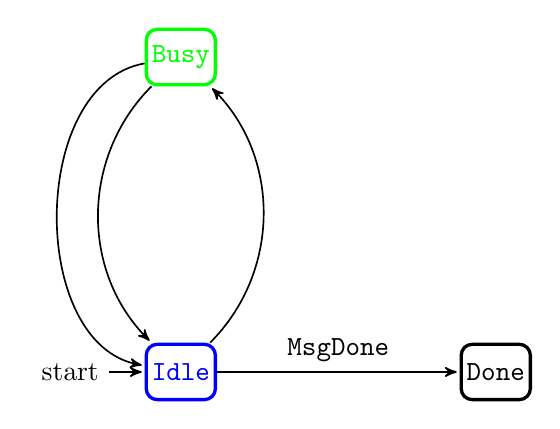
\begin{tikzpicture}[->,>=stealth',shorten >=1pt,auto,node distance=4cm, semithick]
  \tikzstyle{every state}=[fill=red,draw=none,text=white]
  \node[state, blue, initial]                                     (Idle)       {\Idle};
  \node[state, right of=Idle]                                     (Done)       {\Done};
  \node[state, green, above of=Idle]                              (Busy)     {\Busy};

  \draw (Idle)         edge[]                          node{\MsgDone}           (Done);
  \draw (Idle)         edge[right, bend right=45]      node{\SubmitTx}          (Busy);
  \draw (Busy)         edge[left, bend right=45]       node[below = 3mm]{\AcceptTx}          (Idle);
  \draw (Busy)         edge[left, bend right=80]       node[above = 3mm]{\RejectTx}          (Idle);
\end{tikzpicture}

Messages of the protocol:
\begin{description}
\item [\SubmitTx{} {\boldmath $(t)$}]
      The client submits a transaction.
\item [\AcceptTx]
      The server accepts the transaction.
\item [\RejectTx{} {\boldmath $(reason)$}]
      The server rejects the transactions and replies with the $reason$.
\item [\MsgDone]
      The client terminates the mini protocol.
\end{description}

\section{Node-to-Node Transaction Submission Protocol}
\hsref{ouroboros-network/src/Ouroboros/Network/Protocol/TxSubmission/Type.hs}
\label{tx-submission-protocol}
\newcommand{\TxIdsBlocking}   {\state{TxIdsBlocking}}
\newcommand{\TxIdsNonBlocking}{\state{TxIdsNonBlocking}}
\newcommand{\Txs}             {\state{Txs}}
\newcommand{\RequestTxIdsNB}  {\trans{RequestTxIdsNonBlocking}}
\newcommand{\RequestTxIdsB}   {\trans{RequestTxIdsBlocking}}
\newcommand{\ReplyTxIds}      {\trans{ReplyTxIds}}
\newcommand{\RequestTxs}      {\trans{RequestTxs}}
\newcommand{\ReplyTxs}        {\trans{ReplyTxs}}

\subsection{Description}
The node-to-node transaction submission protocol is used to transfer transactions between full nodes.
The protocol follows a pull-based strategy where the initiator asks for new transactions and the responder
replies with the transactions.
It is suitable for a trustless setting where both sides need to guard against resource consumption attacks from
the other side.
The local transaction submission protocol, which is used when the server trusts a local client,
is described in Section \ref{local-tx-submission-protocol}.
The implementation of the node-to-node transaction mini protocol is based on a generic mini protocol framework
(the same as for all other mini protocols).
For technical reasons however the roles of the initiator and the responder are reversed with respect to
the way the other mini protocols are implemented in the frame work.
In other words: The Server is the initiator and ask for new transactions
and the Client is the responder and replies with the transactions.
\subsection{State machine}

\begin{tabular}{|l|l|}
  \hline
  \multicolumn{2}{|c|}{Agency} \\ \hline
  Server has Agency & \Idle \\  \hline
  Client has Agency & \TxIdsBlocking, \TxIdsNonBlocking, \Txs \\ \hline
\end{tabular}

\begin{figure}[h]
\begin{tikzpicture}[->,>=stealth',shorten >=1pt,auto,node distance=4.5cm, semithick]
  \tikzstyle{every state}=[fill=red,draw=none,text=white]
  \node[state, blue, initial](A) at ( 0,  0) {\Idle};
  \node[state]               (B) at ( 8, -4) {\Done};
  \node[state, green]        (C) at ( 4, -4) {\TxIdsBlocking};
  \node[state, green]        (D) at (-4, -4) {\TxIdsNonBlocking};
  \node[state, green]        (E) at ( 0,  4) {\Txs};
  \draw (C)  edge[above]                    node[below]{\MsgDone}                                 (B);
  \draw (A)  edge[left, bend left=45]       node[fill = white, anchor = center]{\RequestTxIdsB}   (C);
  \draw (C)  edge[right, bend left=15]      node[fill = white, anchor = center, above = 2pt]{\ReplyTxIds}     (A);
  \draw (A)  edge[right, bend left=15]      node[fill = white, anchor = center, below = 2pt]{\RequestTxIdsNB} (D);
  \draw (D)  edge[right, bend left=45]      node[fill = white, anchor = center]{\ReplyTxIds}      (A);
  \draw (A)  edge[left, bend right=45]      node[fill = white, anchor = center]{\RequestTxs}      (E);
  \draw (E)  edge[right,bend right=45]      node[fill = white, anchor = center]{\ReplyTxs}        (A);
\end{tikzpicture}
\caption{State machine of the transaction submission protocol.}
\label{tx-submission-automata}
\end{figure}
Messages of the protocol:
\begin{description}
\item [\RequestTxIdsB{} {\boldmath $(ack,req)$}]
      The server asks for new transaction ids and acknowledges old ids.
      The client will block until new transactions are available.
\item [\RequestTxIdsNB{} {\boldmath $(ack,req)$}]
      The server asks for new transaction ids and acknowledges old ids.
      The client immediately replies (possible with an empty list).
\item [\ReplyTxIds{} {\boldmath ($\langle (id, size) \rangle$) }]
      The client replies with a list of available transactions.
      The list contains pairs of transactions ids and the corresponding size of the transaction in bytes.
      In the blocking case the reply is guaranteed to contain at least one transaction.
      In the non-blocking case, the reply may contain an empty list.
\item [\RequestTxs{} {\boldmath ($\langle ids \rangle$)}]
      The server requests transactions by sending a list of transaction-ids.
\item [\ReplyTxs{} {\boldmath ($\langle txs \rangle$})]
      The client replies with a list transaction.
\item [\MsgDone]
      The client terminates the mini protocol.
\end{description}

\begin{tabular}{|l|l|l|l|}
  \hline
  \multicolumn{4}{|c|}{Transition table} \\ \hline
  from state        & message             & parameters                    & to state          \\ \hline\hline
  \Idle             & \RequestTxIdsB      & $ack$,$req$                   & \TxIdsBlocking    \\ \hline
  \TxIdsBlocking    & \ReplyTxIds         & $\langle (id, size) \rangle$  & \Idle             \\ \hline
  \Idle             & \RequestTxIdsNB     & $ack$,$req$                   & \TxIdsNonBlocking \\ \hline
  \TxIdsNonBlocking & \ReplyTxIds         & $\langle (id, size) \rangle$  & \Idle             \\ \hline
  \Idle             & \RequestTxs         & $\langle ids \rangle$         & \Txs              \\ \hline
  \Txs              & \ReplyTxs           & $\langle txs \rangle$         & \Idle             \\ \hline
  \RequestTxIdsB    & \MsgDone            &                               & \Done             \\ \hline
\end{tabular}

\subsection{Client and Server Implementation}
The protocol has two design goals: It must diffuse transactions with high efficiency
and, at the same time, it must rule out
asymmetric resource attacks from the transaction consumer against the transaction provider.

The protocol is based on two pull-based operations.
The transaction consumer can ask for a number of transaction ids and it can use these
transaction ids to request a batch of transactions.
The transaction consumer has flexibility in the number of transaction ids it requests,
whether to actually download the transaction body of a given id
and flexibility in how it batches the download of transactions.
The transaction consumer can also switch between requesting transaction ids and downloading
transaction bodies at any time.
It must however observe several constraints that are necessary for a memory efficient implementation
of the transaction provider.

Conceptually, the provider maintains a limited size FIFO of outstanding transactions per consumer.
(The actual implementation can of course use the data structure that works best).
The maximum FIFO size is a protocol parameter.
The protocol guarantees that, at any time, the consumer and producer agree on the current size of
that FIFO and on the outstanding transaction ids.
The consumer can use a variety of heuristics for requesting transaction ids and transactions.
One possible implementation for a consumer is to maintain a FIFO which mirrors the producers FIFO
but only contains the transaction ids (and the size of the transaction) and not the full transactions.

After the consumer requests new transaction ids, the provider replies with a list of transaction ids and
puts these transactions in its FIFO.
As part of a request a consumer also acknowledges the number of old transactions,
which are removed from the FIFO at the same time.
The provider checks that the size of the FIFO, i.e. the number of outstanding transactions,
never exceeds the protocol limit and aborts the connection if a request violates the limits.
The consumer can request any batch of transactions from the current FIFO in any order.
Note however, that the reply will omit any transactions that have become invalid in the meantime.
(More precisely the server will omit invalid transactions from the reply but they will still be counted in the FIFO
size and they still require a acknowledgement from the consumer).

The protocol supports blocking and non-blocking requests for new transactions ids.
If the FIFO is empty the consumer must use a blocking request
otherwise a non-blocking request.
The producer must reply immediately (i.e. within a small timeout) to a non-blocking request.
It replies with not more then the requested number of ids (possible with an empty list).
A blocking request on the other side, waits until at least one transaction is available.

\section{Handshake Mini Protocol}
\hsref{src/Ouroboros/Network/Protocol/Handshake/Type.hs}
\label{handshake-protocol}
\newcommand{\Propose}{\state{Propose}}
\newcommand{\Confirm}{\state{Confirm}}
\newcommand{\ProposeVersions}{\msg{ProposeVersions}}
\newcommand{\AcceptVersion}{\msg{AcceptVersion}}
\newcommand{\Refuse}{\msg{Refuse}}

\newcommand{\VersionMismatch}{\msg{VersionMismatch}}
\newcommand{\HandshakeDecodeError}{\msg{HandshakeDecodeError}}
\newcommand{\Refused}{\msg{Refused}}

\subsection{Description}
The handshake mini protocol is used to negotiate the protocol version
and the protocol parameters that are used by the client and the server.
It is run exactly once when a new connection is initialised
and consists of a single request from the client and a single reply from the server.
Section \ref{peer-setup-section} explains the live cycle of a connection and the role of
the handshake mini protocol in more detail.

The handshake mini protocol is a generic protocol that can negotiate any kind protocol parameters.
It only assumes that protocol parameters can be encoded to, and decoded from, CBOR terms.
A node, that runs the handshake protocol, must instantiate it with the set of
supported protocol versions and callback functions for handling the protocol parameters.
These callback functions are specific for the supported protocol versions.

\subsection{State machine}

\begin{tabular}{|l|l|}
  \hline
  \multicolumn{2}{|c|}{Agency} \\ \hline
  Client has Agency & \Propose \\ \hline
  Server has Agency & \Confirm \\  \hline
\end{tabular}

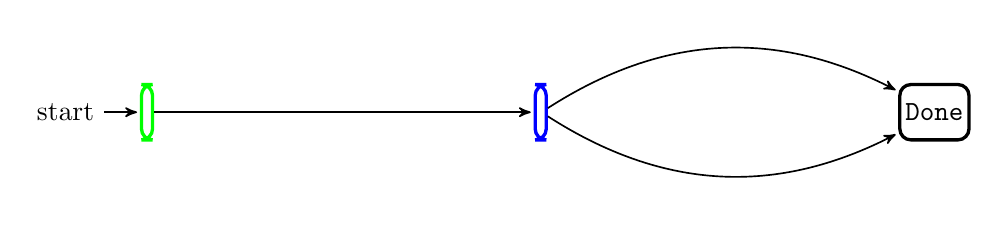
\begin{tikzpicture}[->,>=stealth',shorten >=1pt,auto,node distance=5cm, semithick]
  \tikzstyle{every state}=[fill=red,draw=none,text=white]
  \node[state, green, initial]                                     (Propose)    {\Propose};
  \node[state, blue, right of=Propose]                             (Confirm)    {\Confirm};
  \node[state, right of=Confirm]                                   (Done)       {\Done};

  \draw (Propose)      edge[]      node{\ProposeVersions}          (Confirm);
  \draw (Confirm)      edge[above, bend left]       node{\AcceptVersion}     (Done);
  \draw (Confirm)      edge[below, bend right]      node{\Refuse}            (Done);

\end{tikzpicture}

Messages of the protocol:
\begin{description}
\item [\ProposeVersions{} {\boldmath $(versionTable)$}]
      The client proposes a number of possible versions and protocol parameters.
\item [\AcceptVersion{} {\boldmath $(versionNumber,extraParameters)$}]
      The server accepts $versionNumber$ and returns possible extra protocol parameters.
\item [\Refuse{} {\boldmath $(reason)$}]
      The server refuses the proposed versions.
\end{description}

\begin{tabular}{|l|l|l|l|} \hline
\multicolumn{4}{|c|}{Transition table} \\ \hline
  from        & message/event      & parameters                   & to          \\ \hline\hline
  \Propose    & \ProposeVersions   & $versionTable$              & \Confirm    \\ \hline
  \Confirm    & \AcceptVersion     & $(versionNumber,extraParameters)$ & \Done \\ \hline
  \Confirm    & \Refuse            & $reason$                     & \Done \\ \hline
\end{tabular}

\subsection{Client and Server Implementation}
Section~\ref{included-cddl} contains the CDDL-specification of the binary format of the handshake messages.
The version table is encoded as a CBOR table with the version number as key
and the protocol parameters as value.
The handshake protocol requires that the version numbers ( i.e. the keys) in the version table are unique
and appear in ascending order.
(Note, that CDDL is not expressive enough to precisely specify that requirement on the keys of the CBOR
table. Therefor the CDDL-specification uses a table with keys from 1 to 4 as an example.)

In a run of the handshake mini protocol the peers exchange only two messages:
The client requests to connect with a \ProposeVersions{} message that contains information about
all protocol versions it wants to support.
The server replies either with an \AcceptVersion{} message containing the negotiated
version number and extra parameters or a \Refuse{} message.
The \Refuse{} message contains one of three alternative refuse reasons:
\VersionMismatch{}, \HandshakeDecodeError{} or just \Refused{}.

When a server receives a \ProposeVersions{} message it uses the following algorithm to
compute the response:
\begin{enumerate}
\item
  Compute the intersection of the set of protocol version numbers that the server support
  and the version numbers requested by the client.
\item
  If the intersection is empty:
  Reply with \Refuse(\VersionMismatch) and the list of protocol numbers the server supports.
\item
  Otherwise:
  Select the protocol with the highest version number in the intersection.
\item
  Run the protocol specific decoder on the CBOR term that contains the protocol parameters.
\item
  If the decoder fails:
  Reply with \Refuse(\HandshakeDecodeError), the selected version number and an error message.
\item
  Otherwise: Test the proposed protocol parameters of the selected protocol version
\item
  If the test refuses the parameters:
  Reply with \Refuse(\Refused), the selected version number and an error message.
\item
  Otherwise:
  Encode the extra parameters and
  reply with \AcceptVersion, the selected version number and the extra parameters.
\end{enumerate}
Note, that in step 4), 6) and 8) the handshake protocol uses the callback functions that are specific
for set of protocols that the server supports.
The handshake protocol is designed,
such that a server can always handle requests for protocol versions that it does not support.
The server simply ignores the CBOR terms that represent the protocol parameters of unsupported
version.

The handshake mini protocol runs before the MUX/DEMUX itself is initialised.
Each message is transmitted within a single MUX segment, i.e. with a proper
segment header, but, as the MUX/DEMUX is not yet running the messages must not
be split into multiple segments.  These MUX segments are using a reserved
protocol id $0$ (\texttt{Muxcontrol}).

\section{Pipelining of Mini Protocols}
\label{pipelining}
Protocol pipelining is a technique that improves the performance of some protocols.
The underlying idea is that a client, which wants to perform several requests,
just transmits those requests in sequence without blocking and waiting for the reply from the server.
In the reference implementation, pipelining is used by the clients of all mini protocol except Chain-Sync.
Those mini protocols follow a request-response pattern that is amenable to pipelining such
that pipelining becomes a feature of the client implementation that does not require any
modifications of the server implementation.

As an example, let's consider the Block-Fetch mini protocol.
When a client follows the protocol and sends a sequence of \RequestRange~messages to the server
the data stream from the client to the server will only consist of \RequestRange~messages
(and a final \ClientDone~message) and no other message types.
The server can simply follow the state machine of the protocol and process the messages in turn,
regardless whether the client uses pipelining or not.
The MUX/DEMUX layer (Section~\ref{multiplexing-section}) guarantees
that messages of the same mini protocol are delivered in transmission order,
and therefore the client can determine which response belongs to which request.

The MUX/DEMUX layer also provides a fixed size buffer between the egress of DEMUX and the ingress
of mini protocol thread.
The size of this buffer is a protocol parameter that determines how many messages
a client can send before waiting for a reply from the server (see Section~\ref{mux-flow-control}).
The protocol requires that a client must never cause a overrun of these buffers on a server node.
If a message arrives at the server that would cause the buffer to overrun,
the server treats this case as a protocol violation of the peer
(and closes the connection to the peer).
\hide{
The buffer sizes are listed in Table~\ref{bla} in Section~\ref{blub}.
}

\wip{
  \section{DeltaQ Mini Protocol}

  WIP : Explain DeltaQ measurement back pressure and how we deal with slow
  connection.  See Section % ~\ref{deltaq-discussion}.  The DeltaQ mini
  protocol does not transmit is own messages.  Instead it relies on the time
  stamps that the multiplexing layer (Section~\ref{multiplexing-section}) adds
  to the messages of other mini protocols.
}


\chapter{Multiplexing mini-protocols}
\label{chapter:multiplexer}

\section{The Multiplexing Layer}
\label{multiplexing-section}
Multiplexing is used to run several mini protocols in parallel over
a bidirectional bearer (for example a TCP connection).
Figure~\ref{mux-diagram} ilustrates multiplexing of three mini-protocols over
a single duplex bearer.  The multiplexer guarantees a fixed pairing of
mini-protocol instances, each mini-protocol only communicates with its counter
part on the remote end.

\begin{figure}[ht]
\pgfdeclareimage[height=7cm]{mux-diagram}{figure/mux.png}
\begin{center}
\pgfuseimage{mux-diagram}
\end{center}
\caption{Data flow though the multiplexer and de-multiplexer}
\label{mux-diagram}
\end{figure}


The multiplexer is agnostic to the bearer it runs over, however it assume that
the bearer guarantees an ordered and reliable transport layer\footnote{Slightly
more relaxed property is required: in order delivery of multiplexer segments
which belong to the same mini-protocol.} and it requires the bearer to be
\href{https://www.wikiwand.com/en/Duplex_(telecommunications)\#/Full-duplex}{full-duplex}
to allow simultaneous reads and writes\footnote{Note that one can always pair
two unidirectional bearers to form a duplex bearer, we use this to define
a duplex bearer out of unix pipes, or queues (for intra-process communication
only).}.  The multiplexer is agnostic to the serialisation used by
a mini-protocol (which we specify in section~\ref{chapter:mini-protocols}).
Multiplexer specifies its own framing / binary serialisation format, which is
described in section~\ref{section:wire-format}.  The multiplexer allows to use
each mini-protocol in either direction.

The multiplexer exposes interface which hides all the multiplexer details,
a single mini-protocol communication can be written as if it would only
communicate with its instance on the remote end.  When the muliplexer is
instructed to send bytes of some mini-protocol, it splits the data into
segments, adds a segment header, encodes it and transmits the segments over the
bearer.  When reading data from the network, segment's headers are used
reassemble mini-protocol byte streams.

\subsection{Wire Format}
\label{section:wire-format}

\begin{table}
  \begin{center}
    \begingroup
    \setlength{\tabcolsep}{3pt}
    \begin{tabular}{|c|c|c|c|c|c|c|c|c|c|c|c|c|c|c|c|c|c|c|c|c|c|c|c|c|c|c|c|c|c|c|c|}
      \hline
      0&1&2&3&4&5&6&7&8&9&0&1&2&3&4&5&6&7&8&9&0&1&2&3&4&5&6&7&8&9&0&1 \\ \hline
      \multicolumn{32}{|c|}{Transmission Time} \\ \hline
      \multicolumn{1}{|c|}{$M$}
      &\multicolumn{15}{|c|}{Mini Protocol ID}
      &\multicolumn{16}{|c|}{Payload-length $n$} \\ \hline
      \multicolumn{32}{|c|}{} \\
      \multicolumn{32}{|c|}{Payload of $n$ Bytes} \\
      \multicolumn{32}{|c|}{} \\ \hline
    \end{tabular}
    \endgroup
    \caption{Multiplexer's segment binary encoding, see
    \href{https://input-output-hk.github.io/ouroboros-network/network-mux/Network-Mux-Codec}{Network.Mux.Codec}.}
    \label{segment-header}
  \end{center}
\end{table}

Table~\ref{segment-header} shows the layout of the data segments of the multiplexing protocol
in big-endian bit order.  The segment header contains the following data:
\begin{description}
\item[Transmission Time]
  The transmission time is a time stamp based the lower 32 bits of the sender's monotonic clock with a
  resolution of one microsecond.
\item[Mini Protocol ID] The unique ID of the mini protocol as in
  tables~\ref{table:node-to-node-protocol-numbers}
    and~\ref{table:node-to-client-protocol-numbers}.
\item[Payload Length] The payload length is the size of the segment payload in Bytes.
  The maximum payload length that is supported by the multiplexing wire format is $2^{16}-1$.
  Note, that an instance of the protocol can choose a smaller limit for the size of segments it transmits.
\item[Mode] The single bit $M$ (the mode) is used to distinct the dual instances of a mini protocol.
  The mode is set to $0$ in segments from the initiator, i.e. the side that initially has agency and
  $1$ in segments from the responder.
\end{description}

\subsection{Fairness and Flow-Control in the Multiplexer}
The Shelley network protocol requires that the multiplexer uses a fair
scheduling of the mini protocols.  Haskell implementation of
multiplexer uses a round-robin-schedule of the mini protocols to choose the
next data segment to transmit.  If a mini protocol does not have new data
available when it is scheduled, it is skipped.  A mini-protocol can transmit at
most one segment of data every time it is scheduled and it will only be
rescheduled immediately if no other mini protocol is ready to send data.

From the point of view of the mini protocols, there is a one-message buffer between the egress of
the mini protocol and the ingress of the multiplexer.
The mini protocol will block when it sends a message and the buffer is full.

A concrete implementation of a multiplexer may use a variety of data structures and heuristics to
yield the overall best efficiency.
For example, although the multiplexing protocol itself is agnostic to the underlying structure of
the data, the multiplexer may try to avoid splitting small mini protocol messages into two segments.
The multiplexer may also try to merge multiple messages from one mini protocol into a
single segment.
Note that, the messages within a segment must all belong to the same mini-protocol.

\subsection{Flow-control and Buffering in the Demultiplexer}
\label{mux-flow-control}
The demultiplexer eagerly reads data from the bearer.
There is a fixed size buffer between the egress of the demultiplexer and the ingress of
the mini protocols.
Each mini protocol implements its own mechanism for flow control which guarantees that this buffer
never overflows (see Section~\ref{pipelining}.).
If the demultiplexer detects an overflow of the buffer, it means that the peer violated the
protocol and the MUX/DEMUX layer shuts down the connection to the peer.

\todo[inline]{Specify ingress buffer sizes for each mini-protocol}

\section{Node-to-node and node-to-client protocol numbers}
\noindent\haddockref{Network.Mux.Types}{network-mux/Network-Mux-Types}
\newline\haddockref{Ouroboros.Network.NodeToNode}{ouroboros-network/Ouroboros-Network-NodeToNode}
\newline\haddockref{Ouroboros.Network.NodeToClient}{ouroboros-network/Ouroboros-Network-NodeToClient}

Ouroboros network defines two protocols: \emph{node-to-node} and
\emph{node-to-client} protocols.  \emph{Node-to-node} is used for inter node
communication across the Internet, while \emph{node-to-client} is a inter
process communication, usedy by clients, e.g. a wallet, db-sync, etc.  Each of them consists of a bundle of mini-protocols (see chapter~\ref{chapter:mini-protocols})
consists of a bundle of mini-protocols.  The protocol numbers of both protocols
are specified in tables~\ref{table:node-to-node-protocol-numbers}
and~\ref{table:node-to-client-protocol-numbers}.
\begin{table}[ht]
  \begin{center}
    \begin{tabular}{l|c}
      mini-protocol                                                      & mini-protocol number \\\hline
      \hyperref[handshake-protocol]{Handshake}                           & 0  \\
      \hyperref[chain-sync-protocol]{Chain-Sync} \small{(instantiated to headers)} & 2  \\
      \hyperref[block-fetch-protocol]{Block-Fetch}                       & 3  \\
      \hyperref[tx-submission-protocol]{TxSubmission}                    & 4  \\
      \hyperref[keep-alive-protocol]{Keep-alive}                         & 8  \\
    \end{tabular}
  \end{center}
  \caption{Node-to-node protocol numbers}
  \label{table:node-to-node-protocol-numbers}
\end{table}
\begin{table}[ht]
  \begin{center}
    \begin{tabular}{l|c}
      mini-protocol                                                     & mini-protocol number \\\hline
      \hyperref[handshake-protocol]{Handshake}                          & 0 \\
      \hyperref[chain-sync-protocol]{Chain-Sync} \small{(instantiated to blocks)} & 5 \\
      \hyperref[local-tx-submission-protocol]{Local TxSubmission}       & 6 \\
      \hyperref[local-state-query-protocol]{Local State Query}          & 7 \\
    \end{tabular}
  \end{center}
  \caption{Node-to-client protocol numbers}
  \label{table:node-to-client-protocol-numbers}
\end{table}

\documentclass{article}

\usepackage[utf8]{inputenc}
\usepackage[T1]{fontenc}
\usepackage[british]{babel}
\usepackage[adobe-utopia]{mathdesign}
\usepackage{amsmath}
\usepackage{tikz}
\usepackage{graphicx}
\usepackage{ntheorem}
\usepackage{enumitem}
\usepackage{stmaryrd}
\usepackage{xcolor}
\usepackage[colorlinks,citecolor=blue,linkcolor=blue,anchorcolor=blue,urlcolor=blue]{hyperref}
\usepackage{todonotes}
\usepackage{listings}
\usepackage{colonequals}
\lstset{
  xleftmargin=2pt,
  stepnumber=1,
  belowcaptionskip=\bigskipamount,
  captionpos=b,
  escapeinside={*'}{'*},
  language=haskell,
  tabsize=2,
  emphstyle={\bf},
  commentstyle=\it,
  stringstyle=\mdseries\rmfamily,
  showspaces=false,
  keywordstyle=\bfseries\rmfamily,
  columns=flexible,
  basicstyle=\small\sffamily,
  showstringspaces=false,
  morecomment=[l]\%,
}
\usetikzlibrary{arrows,calc,matrix,shapes}
\tikzset{every scope/.style={>=triangle 60,thick}}
\exhyphenpenalty 10000

\title{Connection Manager State Machine Specification}
\author{Marcin Szamotulski}

\tikzstyle{decision} =
  [ diamond
  , fill=green!255!blue!20
  , text width=4.5em
  , text badly centered
  , node distance=3cm
  , inner sep=0pt
  ]
\tikzstyle{outbound_state} =
  [ rectangle
  , rounded corners
  , fill=blue!60!white!70
  , minimum height=2em
  ]
\tikzstyle{inbound_outbound_state} =
  [ rectangle
  , rounded corners
  , fill=blue!60!red!50
  , minimum height=2em
  ]
\tikzstyle{inbound_state} =
  [ rectangle
  , rounded corners
  , fill=red!50
  , minimum height=2em
  ]
\tikzstyle{impossible_outbound_state} =
  [ rectangle
  , rounded corners
  , fill=blue!40!white!60
  , rounded corners
  , minimum height=2em
  ]
\tikzstyle{line} =
  [ draw
  , -latex'
  ]
\tikzstyle{error} =
  [ rectangle
  , rounded corners
  , fill=red!255!blue!20
  , minimum height=2em
  ]

\def\TCP{\textsf{TCP}}
\def\ipvfour{\textsf{ipv4}}
\def\ipvsix{\textsf{ipv6}}

% States
\def\InitialState{\textbullet}
\def\ReservedOutboundState{\texttt{ReservedOutboundState}}
\def\UnnegotiatedStateOut{\texttt{UnnegotiatedState Outbound}}
\def\UnnegotiatedStateIn{\texttt{UnnegotiatedState Inbound}}
\def\UnnegotiatedStateAny{\texttt{UnnegotiatedState prov}}
\def\OutboundStateUni{\texttt{OutboundState Unidirectional}}
\def\OutboundStateDup{\texttt{OutboundState Duplex}}
\def\OutboundStateAny{\texttt{OutboundState dataFlow}}
\def\DuplexState{\texttt{DuplexState}}
\def\InboundStateUni{\texttt{InboundState Unidirectional}}
\def\InboundStateDup{\texttt{InboundState Duplex}}
\def\InboundStateAny{\texttt{InboundState dataFlow}}
\def\WaitRemoteIdle{\texttt{WaitRemoteIdleState}}
\def\InboundIdleStateUni{\texttt{InboundIdleState Unidirectional}}
\def\InboundIdleStateDup{\texttt{InboundIdleState Duplex}}
\def\InboundIdleStateAny{\texttt{InboundIdleState dataFlow}}
\def\InboundIdleStateUniStar{$\text{\texttt{InboundIdleState Unidirectional}}^\tau$}
\def\InboundIdleStateDupStar{$\text{\texttt{InboundIdleState Duplex}}^\tau$}
\def\TerminatingState{\texttt{TerminatingState}}
\def\TerminatedState{\texttt{TerminatedState}}

% Transitions
\def\Reserve{\textsf{Reserve}}
\def\Connected{\textsf{Connected}}
\def\Accepted{\textsf{Accepted}}
\def\Overwritten{\textsf{Overwritten}}
\def\NegotiatedUniOut{$\text{\textsf{Negotiated}}^\text{\textsf{Unidirectional}}_\text{\textsf{Outbound}}$}
\def\NegotiatedDupOut{$\text{\textsf{Negotiated}}^\text{\textsf{Duplex}}_\text{\textsf{Outbound}}$}
\def\NegotiatedUniIn{$\text{\textsf{Negotiated}}^\text{\textsf{Unidirectional}}_\text{\textsf{Inbound}}$}
\def\NegotiatedDupIn{$\text{\textsf{Negotiated}}^\text{\textsf{Duplex}}_\text{\textsf{Inbound}}$}
% \def\NegotiatedDup{$\text{\textsf{Negotiated}}^\text{\textsf{Duplex}}$}
\def\PromotedToWarmDupLoc{$\text{\textsf{PromotedToWarm}}^\text{\textsf{Duplex}}_\text{\textsf{Local}}$}
\def\PromotedToWarmDupRem{$\text{\textsf{PromotedToWarm}}^\text{\textsf{Duplex}}_\text{\textsf{Remote}}$}
\def\DemotedToColdDupLoc{$\text{\textsf{DemotedToCold}}^\text{\textsf{Duplex}}_\text{\textsf{Local}}$}
\def\DemotedToColdDupRem{$\text{\textsf{DemotedToCold}}^\text{\textsf{Duplex}}_\text{\textsf{Remote}}$}
\def\DemotedToColdUniLoc{$\text{\textsf{DemotedToCold}}^\text{\textsf{Unidirectional}}_\text{\textsf{Local}}$}
\def\DemotedToColdUniRem{$\text{\textsf{DemotedToCold}}^\text{\textsf{Unidirectional}}_\text{\textsf{Remote}}$}
\def\Restart{\textsf{Restart}}
\def\Prune{\textsf{Prune}}
\def\CommitDup{$\text{\textsf{Commit}}^\text{\textsf{Duplex}}$}
\def\CommitUni{$\text{\textsf{Commit}}^\text{\textsf{Unidirectional}}$}
\def\AwakeDupRem{$\text{\textsf{Awake}}^\text{\textsf{Duplex}}_\text{\textsf{Remote}}$}
\def\AwakeUniRem{$\text{\textsf{Awake}}^\text{\textsf{Unidirectional}}_\text{\textsf{Remote}}$}
\def\AwakeDupLoc{$\text{\textsf{Awake}}^\text{\textsf{Duplex}}_\text{\textsf{Local}}$}
\def\Terminate{\textsf{Terminate}}
\def\Timeout{\textsf{Timeout}}

% Peer states
\def\cold{\textit{cold}}
\def\warm{\textit{warm}}
\def\hot{\textit{hot}}
\def\established{\textit{established}}

% Protocol names
\def\keepAlive{\textsf{keep-alive}}
\def\tipSample{\textsf{tip-sample}}

% Component names
\def\ptopgov{\textit{p2p governor}}
\def\mux{\textit{mux}}
\def\inbgov{\textit{inbound protocol governor}}
\def\Inbgov{\textit{Inbound protocol governor}}
\def\connmngr{\textit{connection manager}}
\def\Connmngr{\textit{Connection manager}}
\def\True{\texttt{True}}
\def\False{\texttt{False}}

% Utils

% TODO notes for the implementation
\newcommand{\todoimpl}[1]{\todo[backgroundcolor=red,linecolor=red]{#1}}

\begin{document}
\maketitle

\section{Introduction}
\Connmngr{} is a component responsible for creating or recording
accepted connections and keeping track of their state as we negotiate the
connection and start / stop mnini-protocols on it.  Connection handler drives
through handshake negotiation and starts the multiplexer and will notify the
\connmngr{} about the result of negotiation which triggers a state
transition.  From the point of view of the \connmngr{} it is only
important whether a unidirectional or duplex connection was negotiated.
Unidirectional connections, from node-to-node protocol point of view, are ones
which run either initiator or responder side of mini-protocols exclusively,
while duplex connections can run either or both initiator and responder
protocols.  Note that in the outbound direction (initiator side), it is
\ptopgov{} that is responsible for deciding which set of mini-protocols:
\established{}, \warm{} or \hot{}, is running.  On the inbound side (responder
mini-protocols), we have no choice but to run all of them, so the remote end
can make its decision which mini-protocols set it needs to run.

The \connmngr{} can be run in two \texttt{MuxMode}'s:
\texttt{ResponderMode} or \texttt{InitiatorAndResponderMode}, the
\texttt{InitiatorMode} is not allowed.  The duplex mode:
\texttt{InitiatorAndResponder} is useful for managing connection with external
nodes (\textit{node-to-node protocol}), while \texttt{ResponderMode} is useful
for running a server which responds to local connections
(\textit{node-to-client protocol}).

\Connmngr{} can use at most one \ipvfour{} and at most one \ipvsix{}
address.  It will bind to the correct address depending on the remote address
type (\ipvfour{}/\ipvsix{}).

In this specification we will often need to speak about two nodes communicating
via a \TCP{} connection.  We will often call them local and remote ends of the
connection or local \slash{} remote nodes; we will usually take the
perspective of the local node.

\section{Components} 
\begin{figure}[h]
  \footnotesize
  \def\xa{-2.0}
  \def\xb{2.0}
  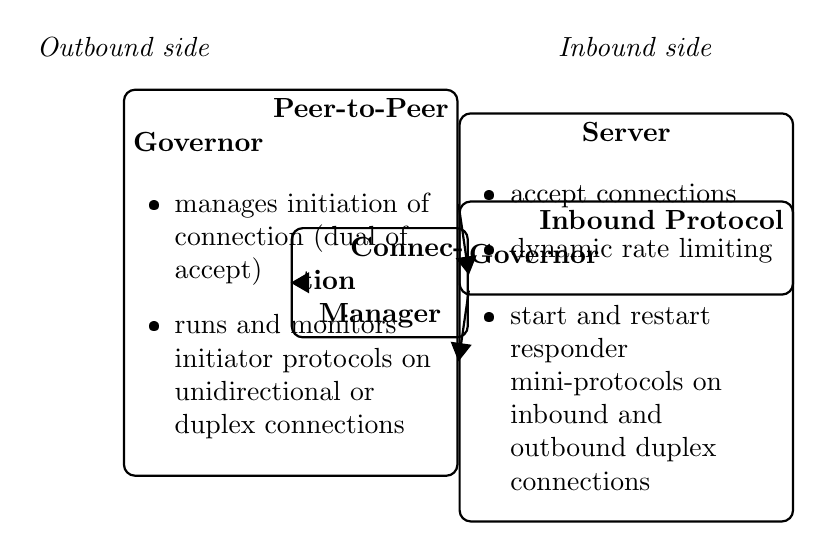
\begin{tikzpicture}
    \node at (-3.25, 0)  {\textit{Outbound side}};
    \node at ( 3.25, 0)  {\textit{Inbound side}};

    \node[rounded corners, rectangle, draw, minimum height=3cm,anchor=east, text width=4cm] (p2p_governor) at (\xa, -3)
     {
       \hfil\textbf{Peer-to-Peer Governor}\hfil\\
       \setlength{\leftmargini}{15pt}
       \begin{itemize}
        \item manages initiation of connection (dual of accept)
        \item runs and monitors initiator protocols on unidirectional or duplex connections
      \end{itemize}
      \vspace{5pt}
      };

    \node[rounded corners, rectangle, draw, anchor=west, text width=4cm] (server) at (\xb, -2)
      {
        \hfill{\textbf{Server}}\hfill
        \vspace{0.2em}
        \setlength{\leftmargini}{15pt}
        \begin{itemize}
          \item accept connections
          \item dynamic rate limiting
        \end{itemize}
        \vspace{5pt}
      };

    \node[rounded corners, rectangle, draw, anchor=west, text width=4cm] (inbound_governor) at (\xb, -4)
      {
        \hfill{\textbf{Inbound Protocol Governor}}\hfill
        \vspace{0.2em}
        \setlength{\leftmargini}{15pt}
        \begin{itemize}
          \item start and restart responder mini-protocols on inbound and
            outbound duplex connections
        \end{itemize}
        \vspace{5pt}
      };

    \node[rounded corners, rectangle, draw, minimum height=1cm, text width=2cm] (connection_manager) at (0, -3)
      {
        \hfil\textbf{Connection}\hfil\\
        \hfil\textbf{Manager}\hfil
      };

    \draw[<-] (p2p_governor)           -- (connection_manager);
    \draw[->] (server.west)            -- (connection_manager.5);
    \draw[->] (connection_manager.355) -- (inbound_governor.west);
  \end{tikzpicture}
\end{figure}

\section{Connection Manager}

\Connmngr{} exposes two methods to register a connection:
\begin{lstlisting}
data Connected peerAddr handle handleError
  -- | We are connected and mux is running.
  = Connected    !(ConnectionId peerAddr) !handle

  -- | There was an error during handshake negotiation.
  | Disconnected !(ConnectionId peerAddr) !(Maybe handleError)

-- | Include outbound connection into 'ConnectionManager'.
requestOutboundConnection
  *'$\coloncolon$'* HasInitiator muxMode ~ True
  *'$\Rightarrow$'* ConnectionManager muxMode socket peerAddr handle handleError m
  *'$\rightarrow$'* peerAddr *'$\rightarrow$'* m (Connected peerAddr handle handleError)

-- | Include an inbound connection into 'ConnectionManager'.
includeInboundConnection
  *'$\coloncolon$'* HasResponder muxMode ~ True
  *'$\Rightarrow$'* ConnectionManager muxMode socket peerAddr handle handleError m
  *'$\rightarrow$'* socket *'$\rightarrow$'* peerAddr *'$\rightarrow$'* m (Connected peerAddr handle handleError)
\end{lstlisting}
The first one asks the \connmngr{} to either connect a peer or if
possible reuse a duplex connection.  The other one allows to register an
inbound connection, which was \texttt{accepted}.  Both methods are blocking
operations and return either an error (handshake negotiation error or
a multiplexer error) or a handle to a \textit{negotiated} connection.

Other methods which are discussed in this specification:

\begin{lstlisting}
-- | Custom either type for result of various methods.
data OperationResult a
    = UnsupportedState !InState
    | OperationSuccess a


-- | Enumeration of states, used for reporting; constructors elided from this
-- specification.
data InState

-- | Unregister an oubound connection.
-- 
unregisterOutboundConnection
  *'$\coloncolon$'* HasInitiator muxMode ~ True
  *'$\Rightarrow$'* ConnectionManager muxMode socket peerAddr handle handleError m
  *'$\rightarrow$'* peerAddr *'$\rightarrow$'* m (OperationResult ())

-- | Notify the 'ConnectionManager' that the remote end promoted us to a /warm
-- peer/; this runs the @PromotedToWarm^{duplex}_{remote}@ transition.
promotedToWarmRemote
  *'$\coloncolon$'* HasInitiator muxMode ~ True
  *'$\Rightarrow$'* ConnectionManager muxMode socket peerAddr handle handleError m
  *'$\rightarrow$'* peerAddr *'$\rightarrow$'* m (OperationResult ())

-- | Unregister outbound connection.  Returns if the operation was successul.
unregisterInboundConnection
  *'$\coloncolon$'* HasResponder muxMode ~ True
  *'$\Rightarrow$'* ConnectionManager muxMode socket peerAddr handle handleError m
  *'$\rightarrow$'* peerAddr *'$\rightarrow$'* m (OperationResult Bool)

-- | Number of connections tracked by the server.
numberOfConnections
  *'$\coloncolon$'* HasResponder muxMode ~ True
  *'$\Rightarrow$'* ConnectionManager muxMode socket peerAddr handle handleError m
  *'$\rightarrow$'* STM m Int
\end{lstlisting}

\section{Connection states}

Each connection is either initiated by \texttt{Inbound} or \texttt{Outbound} side.
\begin{lstlisting}
data Provenance
  = Inbound
  | Outbound
\end{lstlisting}
Each connection negotiates \texttt{dataFlow}:
\begin{lstlisting}
data DataFlow
  = Unidirectional
  | Duplex
\end{lstlisting}
Negotiation of \texttt{DataFlow} is done by the handshake protocol, the final
result depends on two factors: negotiated version and \texttt{InitiatorOnly}
flag which is announced through handshake.  Each connection can be in one
of the following states:
\begin{lstlisting}
data ConnectionState
  -- Connection manger is about to connect to a peer.
  = ReservedOutboundState

  -- Connected to a peer, handshake negotiation is ongoing.
  | UnnegotiatedState Provenance

  -- Inbound connection has been negotiated.
  | InboundState DataFlow

  -- Outbound connection has been negotiated.
  | OutboundState DataFlow

  -- Connection runs in duplex mode: either outbound connection negotiated
  -- 'Duplex' data flow, or 'InboundState Duplex' was reused.
  | DuplexState

  -- Connection has terminated; socket is released, thread running the
  -- connection is closed.  For some small delay the connection is kept in this
  -- state until the kernel releases all the resources.
  | TerminatingState

  -- Connection is removed from connection manager map, at this point the
  -- connection manager can create a new connection to that peer.
  | TerminatedState
\end{lstlisting}
The above type is a stripped version of what is implemented.  The real
implementation tracks more detail, e.g. connection id (the quadruple of ip
addresses and ports), multiplexer handle, etc.

\begin{figure}[p]
  {\hspace{-3cm}\begin{tikzpicture}[scale=0.66]
    \node                         (init)                               at ( 2,   2)     {\small\InitialState};
    \node[inbound_outbound_state] (ReservedOutboundState)              at ( 0,-0.25)    {\small\ReservedOutboundState};
    \node[outbound_state,anchor=east] (UnnegotiatedState_Outbound)     at (-1,  -3)     {\small\UnnegotiatedStateOut};
    \node[inbound_outbound_state] (UnnegotiatedState_Inbound)          at ( 5.5, -3)    {\small\UnnegotiatedStateIn};
    \node[inbound_outbound_state,anchor=west] (InboundIdleState_DupDF)    at ( 1, -6.0) {\small\InboundIdleStateDupStar};
    \node[inbound_state,anchor=west] (InboundIdleState_UniDF)             at ( 5, -7.5) {\small\InboundIdleStateUniStar};
    \node[outbound_state,anchor=east]            (OutboundState_UniDF) at (-2, -10.5)   {\small\OutboundStateUni};
    \node[inbound_outbound_state,anchor=east]    (OutboundState_DupDF) at (-1,  -13)    {\small\OutboundStateDup};
    \node[inbound_state,anchor=west] (InboundState_UniDF)              at ( 5, -11)     {\small\InboundStateUni};
    \node[inbound_outbound_state,anchor=west] (InboundState_DupDF)     at ( 1,  -13)    {\small\InboundStateDup};
    \node[inbound_outbound_state] (DuplexState)                        at (-1.5, -21)   {\small\DuplexState};
    \node[inbound_outbound_state] (TerminatingState)                   at ( 3,  -23)    {\small\TerminatingState};
    \node[inbound_outbound_state] (TerminatedState)                    at ( 3,  -26)    {\small\TerminatedState};


    \draw[->] (init) -- node[fill=white,pos=0.425,above left]{\small\Reserve}                                       (ReservedOutboundState);
    \draw[->] (init) to [out=310, in=90] node[fill=white, above right]{\small\Accepted}                             (UnnegotiatedState_Inbound.30);

    \draw[->] (ReservedOutboundState)          -- node[fill=white,above left] {\small\Connected}                    (UnnegotiatedState_Outbound);
    \draw[->] (ReservedOutboundState)          -- node[fill=white,above right] {\small\Overwritten}                 (UnnegotiatedState_Inbound);

    \draw[->] (UnnegotiatedState_Outbound)     -- node[fill=white,left=-42pt] {\small\NegotiatedUniOut}             (OutboundState_UniDF);
    \draw[->] (UnnegotiatedState_Outbound.290) to [out=-60, in=90]
                                                  node[fill=white,right=-26pt,pos=0.2]{\small\NegotiatedDupOut}     (OutboundState_DupDF.13);

    \draw[->] (UnnegotiatedState_Inbound)          -- node[fill=white,left=-12pt]{\small\NegotiatedDupIn}           (InboundIdleState_DupDF.165);
    \draw[->] (UnnegotiatedState_Inbound)          -- node[fill=white,pos=0.4,right=-28pt]{\small\NegotiatedUniIn}  (InboundIdleState_UniDF);
    \draw[->, dashed] (InboundIdleState_UniDF) -- node[fill=white,right=2pt]{\small\AwakeUniRem}                    (InboundState_UniDF);

    \draw[->, dashed] (InboundState_UniDF) to [out=270, in=20]  node[right=20pt,rotate=90,pos=0.6]{\small\DemotedToColdUniRem}    (TerminatingState.0);
    \draw[->, dashed] (InboundState_DupDF.345) to [out=280, in=90]  node[fill=white,left=10pt,rotate=90,pos=0.2]{\small\DemotedToColdDupRem}
                                                                                                                                  (TerminatingState.30);
    \draw[->]         (InboundIdleState_DupDF.195) -- node[fill=white,pos=0.4]{\small\AwakeDupLoc}                                (OutboundState_DupDF.10);

    \draw[->, dashed] (InboundIdleState_DupDF.200) -- node[fill=white,pos=0.65]{\small\AwakeDupRem}                                           (InboundState_DupDF.160);
    \draw[->]         (OutboundState_DupDF.150) to [out=90,in=-170] node[fill=white,pos=0.45,left=-60pt]{\small\DemotedToColdDupLoc}          (InboundIdleState_DupDF.180);
    \draw[->]         (DuplexState)             to [out=50,in=220]  node[fill=white,pos=0.90,left=18pt,rotate=65]{\small\DemotedToColdDupLoc} (InboundState_DupDF);
    \draw[->]         (InboundState_DupDF)      to [out=-110,in=40] node[pos=0.9,right=22pt,rotate=70]{\small\PromotedToWarmDupLoc}           (DuplexState.10);
    \draw[->, dashed] (DuplexState)             to [out=120,in=-40] node[fill=white,right=10pt,pos=0.1,rotate=90]{\small\DemotedToColdDupRem} (OutboundState_DupDF);
    \draw[->, dashed] (OutboundState_DupDF)     to [out=-90,in=180] node[left,pos=0.05,left=10pt,rotate=80]{\small\PromotedToWarmDupRem}      (DuplexState);

    \draw[->]         (InboundIdleState_DupDF.270) to[out=-80,in=80] node[fill=white,pos=0.15]{\small\CommitDup}                              (TerminatingState.110);
    \draw[->]         (InboundIdleState_UniDF.200) to[out=-90,in=70] node[fill=white,pos=0.5,rotate=80,left=-10pt]{\small\CommitUni}          (TerminatingState.10);

    \draw[->] (OutboundState_UniDF.189)        to [out=270, in=180,pos=0.23,looseness=2]
                                                  node[right=12pt,rotate=88,pos=0.3]{\small\DemotedToColdUniLoc} (TerminatingState.175);

    \draw[->] (TerminatingState) -- node[left]{\Terminate} (TerminatedState);
  \end{tikzpicture}}
  \caption{\textit{Outbound} (blue \& violet) and \textit{inbound} (red \&
  violet) connection states and allowed transitions.  Dashed arrows indicate an
  asynchronous transition, either driven by the decision of a remote peer
  (\DemotedToColdUniRem{} and \DemotedToColdDupRem{}) or the local \connmngr{}
  itself. States which are decorated with $^\tau$ have an associated timeout,
  see~\ref{sec:tr_commit}.}
  \label{fig:statediagram}
\end{figure}

Figure~\ref{fig:statediagram} shows all the transitions between
\texttt{ConnectionState}s.  Blue and violet states represent states of
an \textit{outbound} connection, red and violet represent states of an
\textit{inbound} connection.  Dashed arrows indicate an asynchronous
transitions that are triggered either by remote node or by the connection
manger itself.

Note that the vertical symmetry in the graph corresponds to local / remote
state of the connection:

\begin{table}[h]
  \begin{tabular}[h]{l|l}
    \textit{local connection state} & \textit{remote connection state} \\ [0.3em]
    \hline \\ 
    \UnnegotiatedStateOut{}         & \UnnegotiatedStateIn{}           \\ [0.2em]
    \OutboundStateAny{}             & \InboundStateAny{}               \\ [0.2em]
    \InboundStateAny{}              & \OutboundStateAny{}              \\ [0.2em]
    \DuplexState{}                  & \DuplexState{}                   \\ [0.2em]
  \end{tabular}
\end{table}


\section{Transitions}

\subsection{\Reserve{}}
When \connmngr{} is asked for an outbound connection, it reserves a slot
in its state for that connection.  If any other thread will ask for the same
outbound connection, the \connmngr{} will raise an exception in that thread.
Reservation is done to guarantee exclusiveness for state transitions to
a single outbound thread.

\subsection{\Connected{}}
This transition is executed once an outbound connection successfully performed
\texttt{connect} system call. 

\subsection{\Accepted{} and \Overwritten{}}
Transition driven by \texttt{accept} system call.  Once it returns the
\connmngr{} might either not know about such connection or be in
\ReservedOutboundState{}.  \Accepted{} transition represents the former
situation while the latter is captured by \Overwritten{} transition.

Let us note that if \Overwritten{} transition happened, then on the outbound
side the scheduled \texttt{connect} call will fail.  In this case the
\ptopgov{} will recover, put the peer in a queue of failed peers, and
will either try to connect to another peer or reconnect to that peer after some
delay in which case it would re-use the accepted connection (assuming that
duplex connection was negotiated).

\subsection{\NegotiatedUniOut{} and \NegotiatedDupOut{}}
Once an outbound connection has been negotiated one of \NegotiatedUniOut{} or
\NegotiatedDupOut{} is performed, depending on the result of handshake
negotiation.  Duplex connections are negotiated only for node-to-node protocol
version higher than \texttt{NodeToNodeV\_7}\todoimpl{the exact version number
mightchange} and neither side declared that it is an initiator only.

If duplex outbound connection was negotiated, the \connmngr{} needs to ask the
\inbgov{} to start and monitor responder mini-protocols on the outbound
connection.

This transition is done by the \texttt{requestOutboundConnection}.

\subsection{\NegotiatedUniIn{} and \NegotiatedDupIn{}}
This transition is performed once handshake negotiated a unidirectional or
duplex connection on an inbound connection.  The \textit{inbound protocol
governor} will start all responder protocols (for all \established{}, \warm{}
and \hot{} groups of mini-protocols) and keep monitoring them.

This transition is done by the \texttt{includeInboundConnection}.

\subsection{\AwakeDupLoc{}, \AwakeDupRem{} and \AwakeUniRem{}}
All the awake transitions start either at \InboundIdleStateUni{} or
\InboundIdleStateDup{}.  \AwakeDupRem{} and \AwakeUniRem{} are triggered by
incomming traffic on any of the responders. \AwakeDupLoc{} transition however
is done by \texttt{requestOutboundConnection} on request of \ptopgov{}.

\subsection{\CommitUni{}, \CommitDup{}}\label{sec:tr_commit}
Both commit transition happen after a timeout of inactivity.  They transition
to \TerminatingState{} (closing the bearer).  For duplex connections a normal
shutdown procedure goes through \InboundStateDup{} via \CommitDup{} - which
gave the name to this transitions.

\subsection{\DemotedToColdUniLoc{}}
This transition is driven by the \ptopgov{}: when it decides to demote the peer
to \cold{} state.  This transition should trigger a normal \TCP{} termination,
via \texttt{close} call: we started the connection, and thus we are in position
to close it.

This transition is realised by \texttt{unregisterOutboundConnection}.

\subsection{\DemotedToColdDupLoc{}}
As above this transition is driven by the local \ptopgov{}, but this time it is
triggered on a connection in \texttt{DuplexState}.  The \connmngr{} will need
to be instructed to change the connection state.

This transition is realised by \texttt{unregisterOutboundConnection}.

\subsection{\PromotedToWarmDupLoc{}}
This transition is driven by the local \ptopgov{} when it promotes a \cold{} peer
to \warm{} state.  This is the case where a \connmngr{} will provide
a handle to an existing connection to the \ptopgov{}.

This transition is realised by \texttt{requestOutboundConnection}.

\subsection{\DemotedToColdUniRem{}, \DemotedToColdDupRem{}}
The \DemotedToColdUniRem{} and the two \DemotedToColdDupRem{} transitions are triggered
when the remote end demotes the local peer to \cold{}.  The \inbgov{} can
notice this when one of the \established{} protocols returns.  It will need to
inform the \connmngr{} that this transition happened.  For the
\DemotedToColdDupRem{} from \InboundStateDup{} there is a potential race
condition on which side will call \texttt{close} first.  For this reason it is
safer to transition to \TerminatingState{}.  For \DemotedToColdUniRem{} we
expect that the remote side will call \texttt{close} as soon as it terminated
all its \established{} mini-protocols.  In this case We transition to
\TerminatingState{}.  Even though it's expected that the remote side, which
initiated the connection, calls close first we simply cannot assume
that.  It's not unlikely that both sides will do simultanous \TCP{} close.
Also even if the remote and ended up in \texttt{TIME\_WAIT} state not us,
re-establishing a \TCP{} connection relies on the initial sequence number of
the new connection to be larger than the previous connection (see~\cite[Chapter
2, \texttt{TIME\_WAIT} section]{stevens2003unix}, \cite[Section
4.2.2.13]{RFC1122}), a property we don't want to relay on (various
implementations might vary). For all these reasons transition to
\TerminatingState{,} which will hold the connection for \texttt{TIME\_WAIT}
interval, is a safer option.

This transitions are realised by \texttt{unregisterInboundConnection}.

\subsubsection{Restarting a mini-protocol}
When the server restarts a responder side of a mini-protocol is not a visible
state transition to the governor but it deserves to be described.  The actions
depend on the state in which is the connection:

\paragraph{\DuplexState{}:}
if any responder side of a mini-protocol returns, we
restart it.  This must be a result of either \warm{} to \hot{}, \hot{} to
\warm{} or a transition to \cold{}.  In \DuplexState{} we don't need to
distinguish them: in either case the local \ptopgov{} is still using this
connection.  Note that even in the case of being demoted to \cold{} (and thus
executing \DemotedToColdDupRem{} transition), we restart all the
mini-protocols.

\paragraph{\InboundStateAny{}:}
in these states we need to distinguish remote transtions between \warm{} and
\hot{} and transtions to \cold{}.  In the latter case a mini-protocol shall be
restarted, in the former the \inbgov{} needs to trigger termination procedure:
await with a timeout for all mini-protocols to terminate, when that happens
check once again whether connection is not in \DuplexState{} and trigger one of
\DemotedToColdDupRem{} or \DemotedToColdUniRem{} transition.

We can distinguish transition remote transitions to \cold{} state from
transitions between \warm{} and \hot{} states simply by noticing that an
\established{} mini-protocol terminated.

This transition is implemented with the help of \texttt{isInDuplexState}.

\subsection{\PromotedToWarmDupRem{}}
This transition is triggered by the remote peer, and thus is asynchronous.  The
\inbgov{} can notice it by observing multiplexer ingress side of \established{}
mini-protocols.\footnote{The \texttt{network-mux} library allows to start
mini-protocols lazily, as soon a message for the given mini-protocol is
registered by demultiplexer. For the lazily started mini-protocols the
transtion from \texttt{StatusStartOnDemand} to \texttt{StatusRunning} captures
the state change we are looking for in \PromotedToWarmDupRem{} transition.}
It then should notfiy the \connmngr{}.

This transitions are realised by \texttt{promotedToWarmRemote}.

\subsection{\Prune{} transitions}
First let us note that a connection in \InboundStateDup{}, could have been
initiated by either side.  This means that even though a node might have not
accepted any connection it could end up serving peers and possible go beyond
server hard limit and thus exceed the number of file descriptors.  This is
thanks to the path:
\begin{itemize}
  \item[] \Connected{},
  \item[] \NegotiatedDupOut{},
  \item[] \PromotedToWarmDupRem{},
  \item[] \DemotedToColdDupLoc{}
\end{itemize}
which leads from the initial state \InitialState{} to \InboundStateDup{}, the
same state in which accepted duplex connections end up.  Even though the server
rate limits connections based on how many connections are in this state, we
could end up exceeding server hard limit.

To solve this problem, when a connection is transitioned from 
\DuplexState{} to \InboundStateDup{} (via \DemotedToColdDupLoc{}) the
\connmngr{} will check if we the server hard limit was exceeded.  If that
happened, the \connmngr{} will reset a connection.

If we keep the number of \established{} peers to be smaller than the server
hard limit, we should never need to reset a connection in \DuplexState{}.

We prefer to reset an inbound connections rather than close an outbound
connection because from systemic point of view, outbound connections are more
valuable than inbound ones.

The \textit{inbound protocol governor} is in position to make an educated
decision which connection to reset.  Initially, we aim for a decision driven by
randomness, but other choices are possible\footnote{We can take into account
whether we are \hot{} to the remote end, or for how long we have been \hot{} to
to the remote node.} and the implementation should allow to easily extend the
initial choice.

\subsection{\TerminatingState{} and \TerminatedState{}}
After a connection was closed we keep it in \TerminatingState{} for some time.
This allows for the kernel to release all the resources (addresses).  After
this fixed timeout the connection is removed from the \connmngr{} state,
which we explicitely signify in this specification as \TerminatedState{}.

From operational point of view it's important that connections are not held in
\texttt{TIME\_WAIT} state for too long.  This would be problematic when
restarting a node (without rebooting the system) (e.g. when adjusting
configuration).  The \connmngr{} makes sure that it closes outbound
connections as soon as it can, which means it will only held its outbound
connections in \texttt{TIME\_WAIT} state.  The system setting for
\texttt{TIME\_WAIT} delay is well designed for various network conditions, for
example on Linux it is \texttt{60s}.  To avoid this problem for local relays,
the \connmngr{} can be configured to use ephemeral port for specific
outbound connections.

\subsection{Protocol errors}
If a mini-protocol errors, on either side, connection will be reset (as opposed
to \texttt{close}), and put in \TerminatedState{}.  This can possibly happen in
any connection state.

{\small
Note for implementation: reseting conndtion should be the default.  It can be
set with \texttt{SO\_LINGER} option with a zero linger interval.  This will
cause \texttt{close} call to include \texttt{RST} \TCP{} header.  There are
only two cases where we need \texttt{close} rather than \texttt{reset}:
\DemotedToColdUniLoc{} and \DemotedToColdDupLoc{}.
}

\section{\textit{Outbound} connection}

The state of a connection when \texttt{includeoutboundConnection} is called
which leads to either \OutboundStateUni{} or \DuplexState{} must be either:
\ReservedOutboundState{}, \UnnegotiatedStateIn{} or
\InboundStateDup{}.  If the initial state is \UnnegotiatedStateIn{} then the
the result depends on the negotiation.  If \texttt{Unidirectional} connection was
negotiated \texttt{includeoutboundConnection} must error, if \texttt{Duplex}
connection was negotiated it can use the egress side of this connection leading
to \DuplexState{}.

\paragraph{\textnormal{initial state (\InitialState{})}:} the \connmngr{} does not have
  a connection with that peer.  The  connection is put \ReservedOutboundState{}
  before \connmngr{} connects to that peer;

\paragraph{\UnnegotiatedStateIn{}:} if the \connmngr{} accepted
  a connection from that peer, handshake is ongoing;
  \texttt{requestOutboundConnection} will await until the connection state
  changes to \InboundStateAny{}.

\paragraph{\InboundStateUni{}:} if \texttt{requestOutboundConnection} finds
a connection in this state it will error.

\paragraph{\InboundStateDup{}:} if \connmngr{} accepted connection from
  that peer and handshake negotiated a \texttt{Duplex} data flow;

\paragraph{\TerminatingState{}:} block until \TerminatedState{} and start from
the initial state.

\paragraph{\textnormal{Otherwise}:} if \connmngr{} is asked to connect to
peer and there exists a connection which is in any other state, e.g.
\UnnegotiatedStateOut{}, \OutboundStateAny{}, \DuplexState{}, \connmngr{} signals the caller with an error, see
section~\ref{sub:includeOutboundConnect}.

Figure~\ref{fig:outbound_flow} shows outbound connection state evolution.  This
shows the exact steps and decisions that \texttt{requestOutboundConnection}
needs to make.

\begin{figure}[p]
  \footnotesize{\begin{tikzpicture}[scale=0.8]
    \node[decision]               (init)      at (0,0) {Has a connection to that peer?};
    \node[inbound_outbound_state] (not_found) at (-5, 0) {\ReservedOutboundState{}};

    % Connection not found flow
    \draw[->] (init) -- node[above] {\textbf{no}}  (not_found);
    \node[outbound_state] (connected) at (-5, -3) {\UnnegotiatedStateOut{}};
    \draw[->] (not_found) -- node[left] {\textbf{\texttt{connect}}} (connected);

    % This may be influenced by `initiator only` flag or version of the connection.
    \node[decision]               (handshake_decision_outbound) at (-5, -6.5) {Which data flow was negotiated?};
    \node[outbound_state]         (outbound_unidf)              at (-8, -9)   {\OutboundStateUni{}};
    \draw (connected) -- node[left] {\textbf{\textbf{handshake}}} (handshake_decision_outbound);

    \node[inbound_outbound_state] (outbound_dupdf)             at (-8, -11)  {\OutboundStateDup{}};
    \draw[->] (handshake_decision_outbound.west) -| node[left, near end] {\texttt{Unidirectional}} (outbound_unidf);
    \draw[->] (handshake_decision_outbound) |- node[right, near start] {\textbf{\texttt{Duplex}}} (outbound_dupdf);

    % Connection found flow

    \node[decision] (found) at (0, -5)     {What is the current state?};
    \draw (init) -- node[right] {\textbf{yes}} (found);

    \node[inbound_outbound_state,anchor=west] (reserved_outbound) at (1, -8)  {\ReservedOutboundState};
    \node[error,anchor=west]                  (termination_c)     at (4, -9) {\textbf{error \texttt{ConnectionExists}}};
    \draw   (found.south)       |- (reserved_outbound);
    \draw[] (reserved_outbound) |- (termination_c);

    \node[inbound_outbound_state,anchor=west] (unnegotiated_inbound) at (1, -10) {\UnnegotiatedStateIn};
    \draw (found.south) |- (unnegotiated_inbound.west);
    \draw[->] (unnegotiated_inbound) to[out=90,in=0] node[above right] {\textbf{await}} (found.350);

    \node[inbound_state,anchor=west] (inbound_unidf) at (1, -11) {\InboundStateUni};
    \node[error,anchor=west] (termination_unidf) at (4, -12) {\textbf{error \texttt{ForbiddenConnection}}};
    \draw (found.south) |- (inbound_unidf);
    \draw[] (inbound_unidf) |- (termination_unidf);

    \node[inbound_outbound_state,anchor=west] (inbound_dupdf) at (1, -13) {\InboundStateDup};
    \node[inbound_outbound_state,anchor=west] (duplex)        at (4, -14) {\DuplexState};
    \draw (found.south) |- (inbound_dupdf);
    \draw[->] (inbound_dupdf) |- (duplex);


    \node[impossible_outbound_state,anchor=west] (outbound_uni) at (1, -15) {\OutboundStateUni};
    \draw (found.south) |- (outbound_uni);
    \node[error,anchor=west] (termination_outuni) at (4, -16) {\textbf{error \texttt{ConnectionExists}}};
    \draw (outbound_uni) |- (termination_outuni.west);

    \node[impossible_outbound_state,anchor=west] (duplex_imp)   at (1, -17) {\DuplexState};
    \draw (found.south) |- (duplex_imp);
    \node[error,anchor=west] (termination_dupuni) at (4, -18) {\textbf{error \texttt{ConnectionExists}}};
    \draw (duplex_imp) |- (termination_dupuni.west);

    \node[inbound_outbound_state,anchor=west] (terminating) at (1, -19) {\TerminatingState};
    \draw (found.south) |- (terminating);
    \draw[->] (terminating.0) to [out=0,in=0] node[above right,pos=0.4] {\textbf{await}} (found.10);

    \node[inbound_outbound_state,anchor=west] (terminated)  at (1, -21) {\TerminatedState - not observable};

  \end{tikzpicture}}
  \caption{\textit{Outbound} connection flow graph}
  \label{fig:outbound_flow}
\end{figure}

\subsection{\OutboundStateDup{} and \DuplexState{}}
Once an outbound connection negotiates \texttt{Duplex} data flow it transfers
to \OutboundStateDup{}.  At this point we need to start responder protocols.
This means that the \connmngr{} needs a way to inform server (which
accepts and monitors inbound connections), to start the protocols and monitor
that connection.  This connection will transitioned to \DuplexState{} only once
we notice incoming traffic on any of \established{} protocols.

The implementation is using
\href{https://github.com/input-output-hk/ouroboros-network/blob/coot/connection-manager/ouroboros-network-framework/src/Ouroboros/Network/ConnectionManager/Server/ControlChannel.hs\#L123}{\texttt{TBQueue}}.
Server is using this channel for monitoring inbound connections which includes
starting responder protocols.

\subsection{Termination}\label{sec:outbound_termination}

When \ptopgov{} demotes a peer to \cold{} state an outbound
connection needs to transition either from \OutboundStateUni{} to
\TerminatingState{} or from \DuplexState{} to \InboundStateDup{}.  To
support that the \connmngr{} exposes a method:
\begin{lstlisting}
unregisterOutboundConnection *'$\coloncolon$'* peerAddr *'$\rightarrow$'* m ()
\end{lstlisting}
This method performs \DemotedToColdUniLoc{} or
\DemotedToColdDupLoc{} transition. In the former case it will shut down the
multiplexer and close the \TCP{} connection, in the latter case, beside
changing the connection state, it will also trigger \Prune{} transitions if
the number of inbound connections becomes above the limit.

\subsection{Connection manager methods}
\subsubsection{\texttt{requestOutboundConnection}}\label{sub:includeOutboundConnect}
\begin{tabular}[h]{ll}
  \textit{State}           & \textit{Action} \\\hline\\[2pt]
  \InitialState{}          &
    \begin{minipage}[t]{8cm}
      \begin{itemize}
        \item \ReservedOutboundState{},
        \item \Connected{},
        \item start connection thread (handshake, \mux{})
        \item \NegotiatedUniOut{} or \NegotiatedDupOut{}
      \end{itemize}
    \end{minipage}
    \vspace{8pt}\\
  \ReservedOutboundState{} & error \texttt{ConnectionExists} \\[8pt]
  \UnnegotiatedStateOut{}  & error \texttt{ConnectionExists} \\[8pt]
  \UnnegotiatedStateIn{  } &
    \begin{minipage}[t]{7cm}
      await for \InboundStateAny{}, if negotiated duplex connection
      transition to \DuplexState{}, otherwise error
      \texttt{ForbiddenConnection}
    \end{minipage}
    \vspace{8pt}\\
  \OutboundStateAny{}      & error \texttt{ConnectionExists} \\[8pt]
  \DuplexState{}           & error \texttt{ConnectionExists} \\[8pt]
  \TerminatingState{}      & await for \TerminatedState{}    \\[8pt]
  \TerminatedState{}       & can be treated as initial state \\[8pt]
\end{tabular}

\subsection{\texttt{unregisterOutboundConnection}}
\begin{tabular}[h]{ll}
  \textit{State}           & \textit{Action} \\\hline\\[2pt]
  \InitialState{}          & \texttt{no-op} \\[8pt]
  \ReservedOutboundState{} & error \texttt{ForbiddenOperation} \\[8pt]
  \UnnegotiatedStateOut{}  & error \texttt{ForbiddenOperation} \\[8pt]
  \UnnegotiatedStateIn{}   & error \texttt{ForbiddenOperation} \\[8pt]
  \OutboundStateUni{}      & \DemotedToColdUniLoc{} \\[8pt]
  \OutboundStateDup{}      & \DemotedToColdDupLoc{} \\[8pt]
  \DuplexState{}           & prune connections and run \DemotedToColdDupLoc{} \\[8pt]
  \TerminatingState{}      & \texttt{no-op} \\[8pt]
  \TerminatedState{}       & \texttt{no-op} \\[8pt]
\end{tabular}
The choice between \texttt{no-op} and error is solved by the followin rule: if
the calling component (e.g. \ptopgov{}), is able to keep its state in
a consistent state with \connmngr{} then use \texttt{no-op}, otherwise
error.  Since both \inbgov{} and \ptopgov{} are using \mux{} to track the state
of the connection its actually impossible that the state would be inconsistent.

\section{\textit{Inbound} connection}
Initial states for inbound connection is either:
\begin{itemize}
  \item The initial state: \InitialState{};
  \item \ReservedOutboundState{}
    This can happen when
    \begin{center}
      \texttt{requestOutboundConnection}
    \end{center}
    reserves a connection with \ReservedOutboundState{}, but before it calls
    \texttt{connect} the \texttt{accept} call returned.  In this case, the
    \texttt{connect} call will fail and, as a consequence,
    \texttt{requestOutboundConnection} will fail too.  Any mutable variables
    used by it can be disposed, since there is no thread that could be blocked
    on it: if there was another thread that asked for an oubound connection
    with that peer it would see \ReservedOutboundState{} and it throw
    \texttt{ConnectionExists} exception.

    To make sure that this case is uncommon, we need to guarantee that the
    \connmngr{} does not block between putting the connection in the
    \ReservedOutboundState{} and calling the \texttt{connect} system call.
\end{itemize}

\begin{figure}[h]
  \footnotesize{\begin{tikzpicture}[scale=0.8]
    \node[inbound_outbound_state,draw] (reserved_outbound)    at (-4, 0) {\ReservedOutboundState};
    \node[inbound_outbound_state,draw] (unnegotiated_inbound) at (0, -2)  {\UnnegotiatedStateIn};
    \draw[->] (reserved_outbound) -- (unnegotiated_inbound);

    \node[decision] (handshake_decision_inbound) at (0, -5) {Which data flow was negotiated?};
    \draw (unnegotiated_inbound) -- (handshake_decision_inbound);
    \node[inbound_state]          (inbound_unidf) at (-3, -8) {\InboundStateUni{}};
    \node[inbound_outbound_state] (inbound_dupdf) at (3,  -8) {\InboundStateDup{}};
    \draw[->] (handshake_decision_inbound.west) -| node[left, near end]{\textbf{\texttt{Unidirectional}}} (inbound_unidf);
    \draw[->] (handshake_decision_inbound.east) -| node[right,near end]{\textbf{\texttt{Duplex}}}         (inbound_dupdf);

    \node[inbound_outbound_state] (duplex) at (3, -11) {\DuplexState{}};
    \draw[->] (inbound_dupdf) -- node[right]{\textbf{\texttt{requestOutboundConnection}}} (duplex);
  \end{tikzpicture}}
  \caption{\textit{Inbound} connection flow graph, where both bordered states:
  \ReservedOutboundState{} and \UnnegotiatedStateIn are initial states.}
\end{figure}

\subsection{Server}

The server constists of two components: an accept loop and an \inbgov{}.  The
accept loop is using \texttt{includeInboundConnnection} on incoming
connections, while the \inbgov{} tracks the state of responder side of all
mini-protocols, and is responsible for starting and restarting mini-protocols
as well as detecting usage of them to support the \PromotedToWarmDupRem{}
transition and detecting termination to support the \DemotedToColdUniRem{}
transition.

The \inbgov{} will alway start / re-start all the mini-protocols using
\texttt{StartOnDemand} strategy.  When the multiplexer detects
any traffic on its ingress queues corresponding to responder protocols, the
\inbgov{} will schedule \PromotedToWarmDupRem{} transition with
\texttt{promotedToWarmRemote}.

We detect \DemotedToColdUniRem{} transition as soon as all respnder
mini-protocol are idle for a configurable delay (called
\texttt{serverRespondersIdleTimeout}).  One must use timeout, since it might
happen that a mini-protocol termination message arrives before initial message
of any other mini-protocols, for example when a connection starts and a node is
immediately promoted to \hot{} peer, it might happen that the termination message of
a \warm{} protocol (e.g. \tipSample{}) arrives before initial message of
the \keepAlive{} protcol.

Once \DemotedToColdUniRem{} transition is detected, the \inbgov{} will notify
the \connmngr{} using:

\begin{lstlisting}
-- | Returns 'True' if succeeds, 'False' if the connection is in 'Duplex'
-- state.
unregisterInboundConnection *'$\coloncolon$'* peerAddr *'$\Rightarrow$'* m (OperationResult Bool)
\end{lstlisting}
Which preforms either:
\begin{itemize}
  \item \DemotedToColdUniRem{}, or
  \item \DemotedToColdDupRem{} transition.
\end{itemize}
The first transition, as well as the case
\[
  \text{\DemotedToColdDupRem:\ \InboundStateDup{}}\rightarrow\text{\TerminatingState{}}
\]
will terminate the connection thread and call \texttt{close} the socket.
Though in this case the connection is unlikely to end in \texttt{TIME\_WAIT}
state, what happens in when a connection is reestablished might depend on the
implementation and sequence number of the initial \texttt{SYN}
packet\cite[Chapter 2, \texttt{TIME\_WAIT} section]{stevens2003unix}.

\subsubsection{Forceful termination}
The \connmngr{} might reset a connection through one of the \Prune{}
transitions.

\subsection{Inbound protocol governor in \texttt{ResponderMode}}
When the \connmngr{} runs in \texttt{ResponderMode} it will only expose
methods to make transition for inbound connections, i.e.
\texttt{includeInboundConnection} and \texttt{unregisterInboundConnection}.

In this case the connection state machine simplifies to:

\subsection{Connection manager methods}
\subsubsection{\texttt{includeInboundConnection}}
\begin{center}
  \begin{tabular}[h]{ll}
    \textit{State}           & \textit{Action} \\\hline\\[2pt]
    \InitialState{}          &
      \begin{minipage}[t]{8cm}
        \begin{itemize}
          \item start connection thread (handshake, \mux{})
          \item \NegotiatedUniIn{} or \NegotiatedDupIn{}
        \end{itemize}
      \end{minipage}
      \vspace{8pt}\\
    \ReservedOutboundState{} &
      \begin{minipage}[t]{8cm}
        \begin{itemize}
          \item \Overwritten{},
          \item start connection thread (handshake, \mux{})
          \item \NegotiatedUniIn{} or \NegotiatedDupIn{}
        \end{itemize}
      \end{minipage}
      \vspace{8pt}\\
    \UnnegotiatedStateAny{}  & \texttt{impossible state} \\[8pt]
    \OutboundStateAny{}      & \texttt{impossible state} \\[8pt]
    \DuplexState{}           & \texttt{impossible state} \\[8pt]
    \InboundStateAny{}       & \texttt{impossible state} \\[8pt]
    \TerminatingState{}      & the same as \InitialState{} \\[8pt]
    \TerminatedState{}       & the same as \InitialState{} \\[8pt]
  \end{tabular}
\end{center}

\subsection{\texttt{unregisterInboundConnection}}
\begin{center}
  \begin{tabular}[h]{lll}
    \textit{State}           & \textit{Action} & \textit{Returned Value}\\\hline\\[2pt]
    \InitialState{}          & \texttt{no-op} & \True \\[8pt]
    \ReservedOutboundState{} & error \texttt{ForbiddenOperation} & - \\[8pt]
    \UnnegotiatedStateAny{}  & error \texttt{ForbiddenOperation} & - \\[8pt]
    \OutboundStateAny{}      & error \texttt{ForbiddenOperation} & - \\[8pt]
    \DuplexState{}           & \DemotedToColdDupRem{}            & \False \\[8pt]
    \InboundStateUni{}       & transition to \TerminatedState{}  & \True \\[8pt]
    \InboundStateDup{}       & transition to \TerminatingState{} & \False \\[8pt]
    \TerminatingState{}      & error \texttt{ForbiddenOperation} & - \\[8pt]
    \TerminatedState{}       & error \texttt{ForbiddenOperation} & - \\[8pt]
  \end{tabular}
\end{center}

\subsection{\texttt{promotedToWarmRemote}}
\begin{center}
  \begin{tabular}[h]{lll}
    \textit{StateIn}         & \textit{StateOut}\\\hline\\[2pt]
    \InitialState{}          & \InitialState{}          \\[8pt]
    \ReservedOutboundState{} & \ReservedOutboundState{} \\[8pt]
    \UnnegotiatedStateAny{}  & \UnnegotiatedStateAny{}  \\[8pt]
    \OutboundStateUni{}      & \OutboundStateUni{}      \\[8pt]
    \OutboundStateDup{}      & \DuplexState{}           \\[8pt]
    \DuplexState{}           & \DuplexState{}           \\[8pt]
    \InboundStateUni{}       & \InboundStateUni{}       \\[8pt]
    \InboundStateDup{}       & \InboundStateDup{}       \\[8pt]
    \TerminatingState{}      & \TerminatingState{}      \\[8pt]
    \TerminatedState{}       & \TerminatedState{}       \\[8pt]
  \end{tabular}
\end{center}
The implmentation might use this method when an established mini-protocol
received a message as a method of detection of remote state transition.  Even
though we currently have only one established mini-protocol (i.e. \textit{keep
alive protocol}),  this method should be idempotent.

\bibliographystyle{abbrv}
\bibliography{connection-manager}
\end{document}

% \hide{
\chapter{Peer Discovery and Peer Selection}
\wip{
  Peer discovery and peer selection are relatively independent for the core components of a node.
  In a first iteration, it may be enough to specify what data is going from
  the peer selection algorithm to
  the core components and what data is going from the core components to the peer selection.
  Also peer discovery and peer selection are relatively independent from each other.
  }

\chapter{Infrastructure}
\label{infrastructure}
\wip{
  WIP: Specific assumptions about the infrastructure that are relevant for the discussion.
}

\section{Internet}
\section{Network Topology}
\section{DNS,NTP}
\section{Topographical distribution of block creating nodes}
\section{TCP}
\section{IP}
MTU
\section{Operating Systems}
\section{Firewall}
\section{Nodes and Hosting}
}

\hide{
\chapter{Haskell}
While the network protocol itself can be implemented in many programming languages,
it has been developed in parallel with a Haskell reference implementation.
In addition to the language agnostic protocol description in the other parts of this document,
this section discusses key aspects of the Haskell implementation.
This section is most useful for people who work with the Haskell reference implementation and
may give some extra insights for anybody who is interested in implementing the
network component.
For understanding the protocol, it is save to skip this section.
\section{Constant Memory Consumption}
\section{The State Machine Framework}
\label{Haskell-state-machine}
}

\hide{
\chapter{Discussion}
\section{Related Work}
\subsection{Other Crypto Currencies}
\subsubsection{PoW Systems}
\subsubsection{PoS Systems}
\subsection{Generic Peer to Peer Systems}
\subsection{Formal Correctness}
}
\wip{
  The correctness of distributed and concurrent systems has been studied intensively for decades.
\begin{description}
\item [Safety properties]
  Prove that a bad thing will never happen.
  \begin{itemize}
  \item Coins cannot be stolen
  \item Preservation of Money
  \item Nodes will not run out of Memory
  \item (Property: Current state is valid) will always hold / never fail
  \end{itemize}
\item[Liveness properties]
  Prove that a desired event will happen.
  \begin{itemize}
  \item Message will be delivered
  \item Consensus will be reached
  \item Transaction will be confirmed
  \item Fairness : the desired event will happen in time. One does not have to wait forever
  \item Starvation
  \item Deadlocks
  \end{itemize}
\item[Temporal logic]
  Tailor made logic for analysing concurrent systems.
  \begin{itemize}
  \item Argue about the temporal order of events in transition systems.
  \item Express safety properties.
  \item Express liveness properties.
  \item Express Fairness.
  \item Prove with model checkers.
  \item Refinement properties.
  \item CTL computation tree logic (safety)
  \item LTL linear time logic (fairness)
  \end{itemize}
\item[Time]
  How does a concurrent system deal with time ?
  \begin{itemize}
  \item Physical clocks / Wall clock time
  \item Logical clocks / Vector clocks / order of events
  \item Order of events : Before , Concurrent, After
  \item Hybrid approaches, Ouroboros, slot-times
  \end{itemize}
\item[Session Types]
     Model protocols and transition systems in a type system.
\item[Pi-calculus]
\item[Process algebras]
\end{description}
}
\hide{
\wip{WIP: Poldercast,etc}
\section{Overview}
}
\section{Design Discussion}
\subsubsection{Why distinguish between node to node and node-to-consumer IPC}
\label{why_distinguish_protocols}
We use two different sets of protocols for these two use cases.

\begin{description}
\item[node-to-node] IPC between nodes that are engaged in the high level Ouroboros
      blockchain consensus protocol.
\item[node-to-consumer] IPC between a Cardano node and a `chain consumer' component such as a
      wallet, explorer or other custom application.
\end{description}

This section describes the differences between those two variants of IPC and why they use
different protocols.

The node-to-node protocol is conducted in a P2P environment
with very limited trust between peers. The node-to-node protocol utilises
store-and-forward over selected \emph{bearers} which form the underlying
connectivity graph. A concern in this setting is asymmetric resource
consumption attacks. Ease of implementation is desirable, but is
subordinate to the other hard constraints.

A node-to-consumer protocol is intended to support blockchain applications
like wallets and explorers, or Cardano-specific caches or proxies. The setting
here is that a consumer trusts a node (a `chain producer') and just wants to
catch up and keep up with the blockchain of that producer. It is assumed that
a consumer only consumes from one producer (or one of a related set of
producers), so unlike in the node-to-node protocol there is no need to choose
between different available chains. The producer may still not fully trust the
consumer and does not want to be subject to asymmetric resource
consumption attacks. In this use case, because of the wider range of
applications that wish to consume the blockchain, having some options that are
easy to implement is more important, even if this involves a trade-off with
performance. That said, there are also use cases where tight integration is
possible and making the most efficient use of resources is more desirable.

There are a number of applications that simply want to consume the blockchain,
but are able to rely on an upstream trusted or semi-trusted Cardano consensus
node. These applications do not need to engage in the full consensus protocol,
and may be happy to delegate the necessary chain validation.

Examples include 3rd party applications that want to observe the blockchain,
examples being business processes triggered by transactions or analytics.  It
may also include certain kinds of light client that wish to follow the
blockchain but not do full validation.

Once one considers a node-to-consumer protocol as a first class citizen then it
opens up opportunities for different system architecture choices.
The architecture of the original Cardano Mainnet release was entirely homogeneous:
every node behaved the same, each trusted nothing but itself and paid the full
networking and processing cost of engaging in the consensus protocol.  In
particular everything was integrated into a single process: the consensus
algorithm itself, serving data to other peers and components such as the wallet
or explorer. If we were to have a robust and efficient node-to-consumer protocol
then we can make many other choices.

With an efficient \emph{local} IPC protocol we can have applications
like wallets and explorers as separate processes. Even for tightly
integrated components it can make sense to run them in separate OS
processes and using associated OS management tools. Not only are the
timing constraints for a consensus node much easier to manage when
it does not have to share CPU resources with chain consumers,
but it enables sophisticated end-users to use operating system features
to have finer control over resource consumption.
There have been cases in production where a highly loaded wallet component takes
more than its allowed allocation of CPU resources and causes the local
node to miss its deadlines.  By giving a consensus node a dedicated
CPU core it becomes easier to provide the necessary hard real
time guarantees. In addition, scaling on multi-core machines is
significantly easier with multiple OS processes than with a
multi-threaded OS process with a shared-heap. This could allow
larger capacity Cardano relay deployments where there are multiple
network facing proxy processes that all get their chain from a single
local consensus node.

With an efficient \emph{network} IPC protocol we can do similar things
but extend it across multiple machines. This permits: large
organisations to achieve better alignment with their security
policies; clusters of relays operated by a single organisation to use
the more efficient (less resource costly) node-to-consumer protocol
instead of the node-to-node protocol; and wallet
or explorer-like applications that need to scale out, and are able to
make use of a trusted node.

\hide{
\section{Requirements}
\section{Threat Vectors}
\wip{
\begin{description}
\item [Generic Attacks against IP networks]
\item [Attacks against a specific implementation of the protocol]
\item [Attacks against a specific configuration of the system]
\item [Attacks against the network protocol itself]
\item [Attacks against Ouroboros]
\item [Clever combinations of the above]
\end{description}
}
\subsubsection{Asymptotic Resource Consumption}
\section{Results from Simulations}
\section{Pub Sub}
\section{Of the Shelf Protocols}
\section{Congestion Control}
\subsection{DeltaQ and Back-pressure}
\label{deltaq-discussion}
\wip{WIP: discuss DeltaQ and Back-pressure}

\section{Meta Requirements}
\subparagraph{Work in Progress}
This document is evolved in parallel with the work on the protocol design and
the reference implementation.

\subparagraph{The Document should be Comprehensive}
\begin{itemize}
\item Top down approach.
\item Provide the big picture.
\item Usable as a reference point for a broader discussion.
\item Cover every aspect that is related to network connections.
\item Every aspect should at least have a place in the table of contents.
  If there are holes and parts that are not covered the document should say what is missing.
\item Stand alone readable with links to where missing pieces can be found.
\end{itemize}

\subparagraph{Detailed}
\begin{itemize}
\item Sufficient details to allow for new independent implementations that are compatible with
the reference implementation
\item Language agnostic (it is save to skip the Haskell specific parts)
\item Design discussions
\end{itemize}
\subparagraph{Structured}
\begin{itemize}
\item Parts of the document should be in a logical connection
\end{itemize}
\subparagraph{Workflow}
}

\appendix
\chapter{CDDL Specification of the Protocol Messages}
\label{CBOR-section}
\hsref{ouroboros-network/src/Ouroboros/Network/Protocol/PingPong/Codec.hs}
\label{included-cddl}
This Sections contains the CDDL\cite{cddl} specification
of the binary serialisation format of the network protocol messages.

To keep this Section in close sync with the actual Haskell implementation
the names of the Haskell identifiers have been reused for the corresponding
CBOR types (with the first letter converted to lower case).
Note, that, for readability, the previous Sections used simplified message identifiers,
for example {\tt RequestNext} instead of {\tt msgRequestNext}, etc.
Both identifiers refer to the same message format.

All transmitted messages satisfy the shown CDDL specification.
However, CDDL, by design, also permits variants in the encoding that are not valid in the protocol.
In particular, the notation ${\tt [} ... {\tt ]}$ in CDDL can be used for both fixed-length
and variable-length CBOR-list, while only one of the two encodings is valid in the protocol.
We add comments in specification to make clear which encoding must be used.

Note that, in the case of the request-response mini protocol (Section~ref{request-response-protocol})
there in only ever one possible kind of message in each state.
This means that there is no need to tag messages at all
and the protocol can directly transmit the plain request and response data.

\wip{TODO: test that haskell(message) => cddl(message) }
\lstinputlisting{messages.cddl}
\bibliographystyle{apalike}
\bibliography{references}

\hide{
\chapter{Key Figures of the Protocol and the P2P Network}
This section list some key figures of the network protocol.
There is a variety of figures that quantify some aspects of the protocol, for example:
\begin{itemize}
\item Configuration parameters that are explicitly set in the protocol.
\item Requirements and performance targets.
\item Implicit assumptions about about network bandwidths, etc.
\item Estimates from simulations and game theoretic results.
\end{itemize}
These figures can be a fixed value, a possible interval, a distribution of values,
or just a rough estimate and typically these figures depend on each other.
The figures in this section are not set in stone, but they should help to give a baseline that helps
to understand the protocol design.

Block chain parameters:\\
\begin{tabular}{p{4cm}p{1cm}p{6cm}p{1cm}} \hline
  maximum block size   & = & 2 M Bytes                                    &  \\ \hline
  slot time            & = & 20s                                          &  \\ \hline
  epoch length         & = & 22600 slots $\simeq$ 5 days                  &  \\ \hline
  intrinsic probability of a fork & = &                                   &  \\ \hline
  K parameter (maximal roll back) & = &                                   &  \\ \hline
\end{tabular}\\

Transaction:\\
\begin{tabular}{p{4cm}p{1cm}p{6cm}p{1cm}} \hline
  size of a transaction                & = &  some K Bytes               &  \\ \hline
  through-put transactions per second   & = &  15                        &  \\ \hline
\end{tabular}\\

Network topology:\\
\begin{tabular}{p{4cm}p{1cm}p{6cm}p{1cm}} \hline
  maximum hops                         & $\le$ &  5                         &  \\ \hline
  maximum number of neighbours          & = &  5                         &  \\ \hline
\end{tabular}

\begin{tabular}{p{4cm}p{1cm}p{6cm}p{1cm}} \hline
  bandwidth stake pool                             & = &  > 100Mbit/s             &  \\ \hline
  bandwidth small stake holder                    & = &  ~ 100Mbit/s             &  \\ \hline
  bandwidth none staking chain consumer          & = &  5                       &  \\ \hline
  latency  between stake pool nodes                & <10 ms                       &  \\ \hline
\end{tabular}\\


\chapter{Nomenclature}
\begin{description}
\item[Adversary / Adversarial Action]
  acting in way to subvert the correct (or performant) operation of the distributed protocol.
  Note that non-performance of certain functions at appropriate times can
  fall into this category.
\item[Core DIF]
  The set of end points that belong to the (major)
  stakepools; (the term DIF taken from RINA\ref{RINA} where it denotes
  a (potentially closed) set of potential participants.
\item[egress,ingress]
\item[head of line blocking]
\end{description}
}


\appendix
\chapter{CDDL Specification of the Protocol Messages}
\label{CBOR-section}
\hsref{ouroboros-network/test/messages.cddl}
\label{included-cddl}
This Sections contains the CDDL~\cite{cddl} specification
of the binary serialisation format of the network protocol messages.

To keep this Section in close sync with the actual Haskell implementation
the names of the Haskell identifiers have been reused for the corresponding
CBOR types (with the first letter converted to lower case).
Note, that, for readability, the previous Sections used simplified message identifiers,
for example {\tt RequestNext} instead of {\tt msgRequestNext}, etc.
Both identifiers refer to the same message format.

All transmitted messages satisfy the shown CDDL specification.
However, CDDL, by design, also permits variants in the encoding that are not valid in the protocol.
In particular, the notation ${\tt [} ... {\tt ]}$ in CDDL can be used for both fixed-length
and variable-length CBOR-list, while only one of the two encodings is valid in the protocol.
We add comments in specification to make clear which encoding must be used.

Note that, in the case of the request-response mini protocol (Section~ref{request-response-protocol})
there is only one possible kind of message in each state.  This means that
there is no need to tag messages at all and the protocol can directly transmit
plain request and response data.

\lstinputlisting{../../ouroboros-network/test/messages.cddl}


\bibliographystyle{apalike}
\bibliography{references}

\end{document}
